\documentclass[a4paper]{article}
% \usepackage[vietnam]{babel}
\usepackage[utf8]{vietnam}
\usepackage{minted}
\usepackage{csvsimple}
\usepackage{cases}
% \usepackage{vntex}
%\usepackage[english,vietnam]{babel}
%\usepackage[utf8]{inputenc}
\usepackage{svg}
\usepackage{float}

%\usepackage[utf8]{inputenc}
%\usepackage[francais]{babel}
\usepackage{a4wide,amssymb,epsfig,latexsym,multicol,array,hhline,fancyhdr}

% \usepackage{amsmath}
\usepackage{amsfonts}
\usepackage{amssymb}
\usepackage{lastpage}
\usepackage[lined,boxed,commentsnumbered]{algorithm2e}
\usepackage{enumerate}
\usepackage{color}
\usepackage{graphicx}

% Standard graphics package
\usepackage{array}
\usepackage{tabularx, caption}
\usepackage{multirow}
\usepackage{multicol}
\usepackage{rotating}
\usepackage{graphics}
\usepackage[a4paper,left=2cm,right=2cm,top=1.8cm,bottom=2.8cm]{geometry}
\usepackage{setspace}
\usepackage{epsfig}
\usepackage{tikz}
\usepackage{indentfirst}
\usepackage{bkthesis}
\usetikzlibrary{arrows,snakes,backgrounds}
\usepackage[unicode]{hyperref}
%can file puenc.def trong thu muc goc de option [unicode] tao ra bookmark bang tieng Viet
\hypersetup{urlcolor=blue,linkcolor=black,citecolor=black,colorlinks=true} 
%\usepackage{pstcol} 								
% PSTricks with the standard color package

\newtheorem{theorem}{{\bf Theorem}}
\newtheorem{property}{{\bf Property}}
\newtheorem{proposition}{{\bf Proposition}}
\newtheorem{corollary}[proposition]{{\bf Corollary}}
\newtheorem{lemma}[proposition]{{\bf Lemma}}


%\usepackage{fancyhdr}
\setlength{\headheight}{40pt}
\pagestyle{fancy}
\fancyhead{} % clear all header fields
\fancyhead[L]{
 \begin{tabular}{rl}
    \begin{picture}(25,15)(0,0)
    \put(0,-8){
\includegraphics[width=8mm, height=8mm]{img/LogoBK.jpg}}
    %\put(0,-8){\epsfig{width=10mm,figure=hcmut.eps}}
   \end{picture}&
	%\includegraphics[width=8mm, height=8mm]{hcmut.png} & %
	\begin{tabular}{l}
		\textbf{\bf \ttfamily Trường Đại học Bách Khoa - ĐHQG TP.HCM}\\
		\textbf{\bf \ttfamily Khoa Khoa học \& Kỹ thuật Máy tính}
	\end{tabular} 	
 \end{tabular}
}
\fancyhead[R]{
	\begin{tabular}{l}
		\tiny \bf \\
		\tiny \bf 
	\end{tabular}  }
\fancyfoot{} % clear all footer fields
\fancyfoot[L]{\scriptsize \ttfamily Hệ thống phòng Tổ chức hành chính}
\fancyfoot[R]{\scriptsize \ttfamily Page {\thepage}/\pageref{LastPage}}
\renewcommand{\headrulewidth}{0.3pt}
\renewcommand{\footrulewidth}{0.3pt}


%%%
\setcounter{secnumdepth}{4}
\setcounter{tocdepth}{3}
\makeatletter
\newcounter {subsubsubsection}[subsubsection]
\renewcommand\thesubsubsubsection{\thesubsubsection .\@alph\c@subsubsubsection}
\newcommand\subsubsubsection{\@startsection{subsubsubsection}{4}{\z@}%
                                     {-3.25ex\@plus -1ex \@minus -.2ex}%
                                     {1.5ex \@plus .2ex}%
                                     {\normalfont\normalsize\bfseries}}
\newcommand*\l@subsubsubsection{\@dottedtocline{3}{10.0em}{4.1em}}
\newcommand*{\subsubsubsectionmark}[1]{}
\makeatother

\begin{document}
\usetikzlibrary{calc}

\begin{titlepage}
\begin{tikzpicture}[remember picture, overlay]
  \draw[line width = 2pt,color=blue] ($(current page.north west) + (2.15cm,-2.15cm)$) rectangle ($(current page.south east) + (-2.15cm,2.15cm)$);
   \draw[line width = 1pt,color=black] ($(current page.north west) + (2.0cm,-2.0cm)$) rectangle ($(current page.south east) + (-2.0cm,2.0cm)$);
\end{tikzpicture}
\begin{center}
TRƯỜNG ĐẠI HỌC BÁCH KHOA - ĐHQG TP.HCM\\
\textbf{KHOA KHOA HỌC VÀ KỸ THUẬT MÁY TÍNH}\\
- - - - - - - - - - - -
\end{center}

\vspace{0.5cm}
\begin{figure}[H]
\begin{center}

\includegraphics[width=3cm]{img/LogoBK.jpg}
\end{center}
\end{figure}
\vspace{0.5cm}

\begin{center}
\begin{tabular}{c}
\multicolumn{1}{c}{\textbf{{\huge ĐỀ CƯƠNG LUẬN VĂN TỐT NGHIỆP }}}\\
~~\\
\hline
\multicolumn{1}{c}{\textbf{{\Large Xây dựng}}}\\\\
\textbf{{\Large Hệ thống Tổ chức hành chính}}\\
\hline
\end{tabular}
\end{center}

\vspace{1cm}
\begin{table}[H]
\begin{tabular}{rlr}
\hspace{5cm} GVHD: & Th.S Nguyễn Thanh Tùng&\\
\\
\hspace{5cm} SV thực hiện: & Nguyễn Quốc Cường & 1610372\\
& Nguyễn Hoàng Nam & 1612115\\
& Nguyễn Xuân Thi & 1613297\\

\end{tabular}
\end{table}
\vspace{3cm}
\begin{center}
{\footnotesize Tp. Hồ Chí Minh, Tháng 12/2019}
\end{center}
\end{titlepage}


% \selectlanguage{vietnamese}
\newpage
\begin{declaration}
Chúng tôi xin cam đoan rằng đề tài luận văn tốt nghiệp: "Xây dựng hệ thống tổ chức hành chính" là do chúng tôi thực hiện dưới sự hướng dẫn của Th.S Nguyễn Thanh Tùng. Tất cả các tham khảo từ
các công trình khác đều được ghi rõ trong mục "Tài liệu tham khảo". Nội dung của luận văn này chưa từng được công bố trước đây dưới bất kì hình thức nào. Nếu có bất kì sai phạm nào, chúng tôi xin chịu hoàn toàn trách nhiệm trước Ban Chủ nhiệm Khoa và Ban Giám hiệu Nhà trường.
\end{declaration}
\newpage
\tableofcontents
\newpage
\listoffigures
\newpage
\listoftables
\newpage
%%%%%%%%%%%%%%%%%%%%%%%%%%%%%%%%%

%%%%%%%%%%%%%%%%%%%%%%%%%%%%%%%%%
\section{Giới thiệu phòng Tổ chức - Hành chính của Đại học Bách Khoa - ĐHQG-HCM}
Ngày nay, trong đời sống xã hội nói chung, các cơ quan quản lý nhà nước và các doanh nghiệp sản xuất kinh doanh nói riêng, con người là một nhân tố cực kỳ quan trọng: bằng sự lao động sáng tạo của mình sẽ thúc đẩy mọi sự phát triển của xã hội. Vì vậy đối với bất kỳ lĩnh vực nào thì con người cũng là trung tâm của mọi sự điều khiển.

Quản lý nhân sự là một trong những bộ phận quan trọng trong tổ chức, đặc biệt là trong các tổ chức lớn trong nước và các tổ chức nước ngoài. Sự thành bại của tổ chức phụ thuộc vào cách thức tổ chức nhân sự có tốt hay không. Trong những năm vừa qua quản lý nhân sự đang dần phát triển mạnh mẽ không những ở các tổ chức nước ngoài mà các tổ chức trong nước cũng đang dần nhận thấy sự quan trọng của tổ chức nhân sự trong tổ chức.

Phòng Tổ chức - Hành chính là một phòng ban quan trọng của Đại học Bách Khoa - ĐHQG-HCM. Phòng có chức năng tham mưu, giúp cho Hiệu trưởng và Đảng Ủy trong việc chỉ đạo, thực hiện công tác tổ chức bộ máy quản lý cán bộ nhà trường theo đúng các chủ trương chính sách của Đảng, Nhà nước và các quy định quy chế của Bộ, Đại học Quốc gia và Nhà trường đã ban hành. Tổ chức giao dịch hành chính, trao đổi thông tin giữa Ban Giám hiệu với các cơ quan khác trong nước và giữa Ban Giám hiệu với các đơn vị, CBCNV, sinh viên trong trường.\\

Các chức năng, nhiệm vụ của phòng Tổ chức - Hành chính:
\begin{itemize}
    \item Nghiên cứu, đề xuất xây dựng bộ máy tổ chức đội ngũ và tổ chức điều hành trong trường.
    \item Xây dựng và hướng dẫn thực hiện các nội quy, quy chế về định biên và quản lý biên chế.
    \item Lập và quản lý hồ sơ về lương, thủ tục đề nghị nâng bậc và điều chỉnh lương hàng năm.
    \item Chỉ đạo và thực hiện công tác bảo vệ chính trị, trật tự an ninh trong khuôn viên trường.
    \item Tổ chức quản lý, lưu trữ hồ sơ lý lịch của CBCNV, bổ sung và nhận xét hàng năm.
\end{itemize}

\section{Các vấn đề hiện tại của phòng Tổ chức - Hành chính}
Phòng Tổ chức - Hành chính, Đại học Bách Khoa - Đại học Quốc gia TP.HCM hiện tại đang lưu trữ và sử dụng dữ liệu dưới dạng các file Microsoft Access, Microsoft Excel, Microsoft Word và một số tài liệu giấy. Cách thức hoạt động này được triển khai từ nhiều năm trước với những ưu điểm như sau:
\begin{itemize}
    \item Vì sử dụng các phần mềm Microsoft Word, Excel nên thân thiện, dễ sử dụng với cán bộ, nhân viên của phòng Tổ chức - Hành chính.
    \item Dễ mở rộng nếu có thêm các nghiệp vụ mới.
    \item Dễ tạo báo cáo, thống kê bằng Microsoft Word, Microsoft Excel.
    \item Nhân viên mới dễ dàng làm quen và sử dụng hệ thống.
\end{itemize}

Tuy nhiên, cách hoạt động này chỉ hiệu quả khi hệ thống còn ít người dùng, dữ liệu còn nhỏ, nghiệp vụ ít, đơn giản. Ở thời điểm hiện tại, khi lượng dữ liệu và các nghiệp vụ mà phòng Tổ chức - Hành chính cần quản lý ngày càng nhiều, thì cách thức hoạt động này thể hiện những hạn chế như sau: 
\begin{itemize}
    \item Các nghiệp vụ như nhập liệu, tính toán, lưu trữ hiện nay được cán bộ phòng Tổ chức - Hành chính thực hiện thủ công nên tốn nhiều thời gian và có thể dẫn đến những sai sót, trùng lặp, thiếu sót.
    \item Dữ liệu ngày càng nhiều, dẫn đến khó khăn trong việc lưu trữ, quản lý, truy xuất.
    \item Không có cơ chế phân quyền cho các cán bộ của phòng, vì vậy có thể dẫn đến các thao tác, hành động vượt quá quyền hạn, ảnh hưởng đến hệ thống. 
    \item Dữ liệu trên website http://www.tchc.hcmut.edu.vn lỗi thời, việc cập nhập dữ liệu lên website khá khó khăn và tốn thời gian.
    \item Cần phải cài đặt các phần mềm mới truy cập được vào hệ thống. Không truy cập được khi sử dụng các thiết bị di động.
    \item Việc trao đổi thông tin trong nội bộ phòng ban và giữa phòng ban với bên ngoài gặp nhiều khó khăn.
    \item Cán bộ, công nhân viên mới phải điền thông tin vào các mẫu lý lịch có sẵn và được cán bộ nhập liệu vào hệ thống một cách thủ công, gây tốn thời gian và có thể dẫn đến sai sót thông tin.
    \item Tốn nhiều chi phí cho việc lưu trữ, sắp xếp, tìm kiếm hồ sơ CBCNV trong kho chứa.
    \item Dễ dẫn đến sai sót khi tính toán, đặc biệt là tính toán tiền lương, điểm thi đua cán bộ... Nếu có sai sót thì sẽ dẫn đến hậu quả nghiêm trọng.
\end{itemize}
\textbf{Kết luận chung:}

Hệ thống phòng Tổ chức - Hành chính của trường Đại học Bách Khoa - Đại học Quốc gia TP.HCM hiện tại đã lỗi thời, gây nhiều khó khăn cho cán bộ, nhân viên nhà trường trong quá trình vận hành và sử dụng. Vì vậy, việc xây dựng hệ thống Tổ chức - Hành chính mới để giải quyết được các các khó khăn hiện tại, bổ sung các tính năng mới, cải thiện công tác quản lý, vận hành công việc của phòng Tổ chức - Hành chính là thực sự cần thiết.
    
\section{Mục tiêu của đề tài}
Mục tiêu của đề tài này là xây dựng một hệ thống thông tin phòng Tổ chức - Hành chính của Đại học Bách Khoa - Đại học Quốc gia TP.HCM với các tính năng như sau:

\begin{itemize}
    \item Quản lý thông tin cán bộ công nhân viên nhà trường, bao gồm các tính năng tìm kiếm, thêm, xoá, sửa, lưu thông tin, nhập dữ liệu từ file Excel,...
    \item Website truyền thông với giao diện đẹp, dữ liệu đầy đủ, update thường xuyên, cung cấp các thông tin mới, quan trọng với cán bộ, sinh viên, người dùng,... 
    \item Tính năng thống kê, tổng hợp, tính điểm thi đua.
    \item Tính năng thống kê, tổng hợp, tính điểm điểm thưởng.
    \item Quản lý bảo hiểm cho cán bộ.
    \item Quản lý các cấp, đơn vị hành chính của nhà trường.
    \item Quản lý quy trình khen thưởng, kỷ luật.
    \item Quản lý lương cán bộ.
    \item Quản lý chức danh, chức vụ của cán bộ.
    \item Quản lý quá trình đào tạo chuyên môn.
    \item Quản lý quá trình công tác trong nước và nước ngoài của cán bộ.
    \item Bồi dưỡng nghiệp vụ cho cán bộ.
    \item Quản lý cán bộ công tác trong và ngoài nước.
    \item Tuyển chọn cán bộ.
    \item Chia sẻ thông tin cho các cán bộ, phòng ban khác.
    \item Quản lý lương, thưởng và các kế hoạch bảo hiểm, trợ cấp của người lao động.
    \item Xuất các báo cáo, thống kê theo yêu cầu và theo định kỳ.
\end{itemize}
\section{Phạm vi đề tài}
Phạm vi các đối tượng mà đề tài hướng đến là:
\begin{itemize}
    \item Cán bộ, nhân viên phòng Tổ chức - Hành chính với vai trò vận hành quản lý hệ thống.
    \item Cán bộ, công nhân viên trường Đại học Bách Khoa - Đại học Quốc gia TP.HCM.
    \item Sinh viên và cựu sinh viên trường Đại học Bách Khoa - Đại học Quốc gia TP.HCM.
    \item Các đơn vị, doanh nghiệp là đối tác của nhà trường.
\end{itemize}
\section{Khó khăn và thử thách}
Các khó khăn, thử thách mà đề tài gặp phải:
\begin{itemize}
    \item Độ ổn định của hệ thống.
    \item Lượng cán bộ sử dụng lớn.
    \item Số lượng nghiệp vụ lớn.
    \item Đầy đủ các chức năng nhưng vẫn phải đảm bảo dễ dàng sử dụng.
\end{itemize}
\section{Phân tích yêu cầu đề tài}
\subsection{Phân quyền người dùng trong hệ thống}
\indent Dựa vào những yêu cầu thực tế của hệ thống và những khảo sát đối với các cá nhân có nhu cầu sử dụng, xây dựng hệ thống Tổ chức hành chính. Nhóm đưa ra các vai trò, người dùng chính trong hệ thống như sau:
\begin{itemize}
    \item Quản trị hệ thống
    \item Cán bộ, nhân viên của trường
    
\end{itemize}
\section{Công nghệ sử dụng}
\subsection{Mô hình Model-View-Controller}
Mô hình Model-View-Controller viết tắt là MVC, là một mô hình được sử dụng rộng rãi trong các dự án phát triển phần mềm hệ thống web. Mô hình được tạo nên từ ba thành phần, mỗi thành phần tương ứng với một chức năng trong mô hình.
\begin{itemize}
    \item Model là bộ phận có nhiệm vụ lưu trữ toàn bộ dữ liệu của ứng dụng. Model chứa tất cả các hàm, phương thức truy vấn trực tiếp với dữ liệu. Bộ phận này là cầu nối giữa hai thành phần Controller và View ở bên dưới. 
    \item View là thành phần giao diện người dùng, thành phần này có nhiệm vụ gửi yêu cầu đến Controller để lấy dữ liệu và hiển thị nội dung lên giao diện.
    \item Controller có nhiệm vụ tiếp nhận yêu cầu từ phía người dùng thông qua View và lấy dữ liệu tương ứng từ Model để trả về cho người dùng
\end{itemize}
\begin{center}
  \captionsetup{type=figure}
  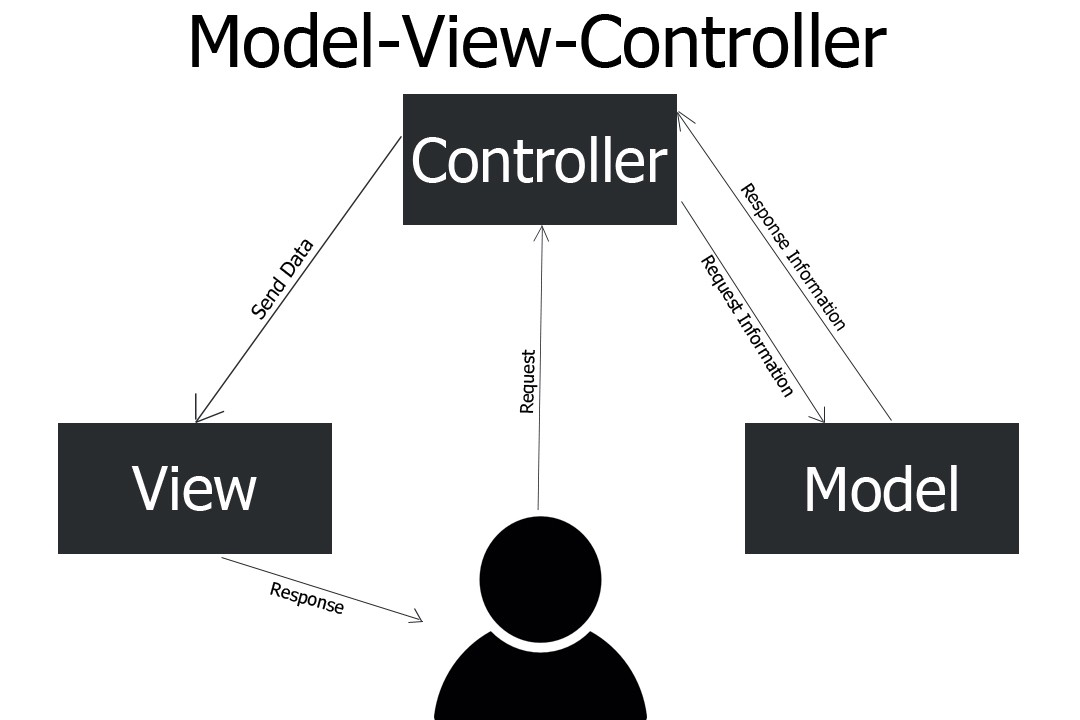
\includegraphics[scale=0.2]{img/mvc.jpg}
  \captionof{figure}{Mô hình MVC}
\end{center}
\indent Hệ thống được chia ra các thành phần riêng biệt với nhau nên trong quá trình kiểm thử sẽ dễ dàng phát hiện và chỉnh sửa lỗi. Bên cạnh đó, việc nâng cấp phần mềm cũng trở nên dễ dàng hơn

\subsection{Ứng dụng đa trang và ứng dụng đơn trang}
Khi phát triển một ứng dụng, có hai kiểu thiết kế phổ biến hiện nay là ứng dụng đa trang (Multi-page Application-MPA) và ứng dụng đơn trang (Single-page Application-SPA). Mỗi kiểu thiết kế có những ưu và nhược điểm riêng phù hợp với các ứng dụng khác nhau. Vì vậy để có thể phát triển ứng dụng một cách hiệu quả, nhà phát triển phải cân nhắc lựa chọn cách thiết kế phù hợp nhất với nhu cầu của ứng dụng của mình.
\subsubsection{Ứng dụng đa trang (Multi-page Application-MPA)}
Ứng dụng đa trang chứa nhiều trang liên kết và các trang con, được điều hướng bằng menu. Ứng dụng đa trang phù hợp với hầu hết các dự án. Ứng dụng đa trang được sử dụng rộng rãi trong nhiều lĩnh vực như thương mại điện tử (amazon.com), e-learning (lynda.com),...\\\\\textit{Ưu điểm:}
\begin{itemize}
    \item Cho phép khả năng mở rộng ứng dụng thông qua menu và thanh tìm kiếm.
    \item Luồng điều hướng dễ theo dõi. 
    \item Hỗ trợ tốt cho SEO.
\end {itemize}
\textit{Nhược điểm:}
\begin{itemize}
    \item Các ứng dụng có nhiều nội dung lớn thường tải chậm, ảnh hưởng đến trải nghiệm của khách hàng.
    \item Khó thích nghi tốt với thiết bị di động.
\end {itemize}
\subsubsection{Ứng dụng đơn trang (Single-page Application-SPA):}
Ứng dụng đơn trang chỉ chứa 1 trang HTML, không có trang bổ sung, chẳng hạng như giới thiệu, liên hệ,...Ứng dụng đơn trang không yêu cầu tải lại trang khi sử dụng, các nội dung sẽ được tải bằng Javascript.\\\\
\textit{Ưu điểm:}
\begin{itemize}
    \item Tốc độ nhanh, do các tài nguyên được tải xuống khi trong suốt quá trình sử dụng.
    \item Có khả năng làm việc với cache tốt, nên hiệu quả khi sử dụng ở chế độ offline.
    \item Thích nghi tốt với thiết bị di động.
\end{itemize}
\textit{Nhược điểm:}
\begin {itemize}
    \item Không tốt cho SEO (các công cụ tìm kiếm). Việc tìm kiếm các nội dung trong ứng dụng đơn trang bằng các công cụ tìm kiếm (google.com, bing.com) thường ít hiệu quả.
    \item Khó khăn trong việc mở rộng.
\end {itemize}
\subsubsection{Kết luận và lựa chọn:}
Nhận thấy hệ thống phòng tổ chức hành chính có những đặc điểm như sau:
\begin {itemize}
    \item Có nhiều nội dung tương đối giống nhau nên việc sử dụng ứng dụng đa trang là không cần thiết.
    \item Hệ thống tập trung vào tác vụ xử lý nên ưu tiên tốc độ cao.
    \item Hệ thống phát triển hỗ trợ hoạt động của phòng tổ chức hành chính do đó không cần quá chú trọng vào SEO.
\end {itemize}

Vì vậy nhóm quyết định sử dụng ứng dụng đơn trang vào ứng dụng phòng tổ chức hành chính.





\subsection{Các thư viện và framework cho Frontend}
Front-end của một ứng dụng được hiểu là phần tương tác trực tiếp với người dùng. Nhà phát triển sử dụng kết hợp các ngôn ngữ như HTML, CSS, JavaScipt,... thiết kế nên giao diện để người dùng có thể xem và tương tác trực tiếp với ứng dụng.

Hiện nay, các ứng dụng có nội dung ngày càng lớn, yêu cầu của người dùng về UI-UX ngày càng cao, gây khó khăn khi phát triển. Vì vậy, các front-end framework ra đời giúp tiết kiệm thời gian lập trình, tối ưu hoá và dễ dàng tạo ra các tương tác thân thiện với người dùng.

Tuy nhiên lại có rất nhiều front-end framework khác nhau, với các tính năng và đặc điểm nổi bật riêng. Vì vậy, nhóm quyết định tìm hiểu các framework phổ biến nhất để từ đó đưa ra sự lựa chọn phù hợp cho ứng dụng của mình.
\subsubsection{React}
React là một thư viện được JavaScipt để phát triển giao diện người dùng, được xây dựng cho các nhà phát triển của Facebook và Instagram.

React nổi lên với xu hướng Single Page Application, đơn giản và dễ dàng phối hợp với những thư viện Javascript khác. Trong báo cáo khảo sát lập trình viên stack-overflow 2019, React đã vươn lên vị trí thứ 2 ở mục các Web Framework phổ biến nhất.

Các đặc điểm chính:
\begin {itemize}
\item Được sử dụng để xây dựng ứng dụng đơn trang
\item React hỗ trợ việc xây dựng những thành phần (components) UI có tính tương tác cao, có trạng thái và có thể tái sử dụng.
\item React không chỉ hoạt động trên phía client, mà còn được render trên server và có thể kết nối với nhau
\end {itemize}

\subsubsection{jQuery}
jQuery là một thư viện JavaScript nhanh, nhỏ và giàu tính năng. Nó làm cho mọi thứ như chuyển đổi và thao tác đối với HTML, xử lý sự kiện, hiệu ứng và Ajax đơn giản hơn nhiều với API dễ sử dụng, hoạt động trên vô số trình duyệt. Với sự kết hợp giữa tính linh hoạt và khả năng mở rộng, jQuery đã thay đổi cách hàng triệu người viết JavaScript.\\

\textit{Đặc điểm và thế mạnh:}
\begin{itemize}
    \item \textbf{Dễ sử dụng:} Đây là lợi thế chính khi sử dụng jquery, nó dễ dàng hơn so với nhiều thư viện javascript chuẩn khác bởi cú pháp đơn giản và bạn chỉ phải viết ít dòng lệnh để tạo ra các chức năng tương tự. Chỉ với 10 dòng lệnh JQuery bạn có thể thay thế cả 20 chục dòng lệnh DOM javaScript, tiết kiệm thời gian của người lập trình.
    \item \textbf{Là một thư viện lớn của javascript:} Thực thi được nhiều chức năng hơn so với các thư viện jascript khác
    \item \textbf{Cộng đồng mã nguồn mở mạnh mẽ:} JQuery đang còn tương đối mới, có một cộng đồng dành thời gian của họ để phát triển các plugin của JQuery. Như vậy có hàng trăm plugin được viết trước đó có sẵn để tải về ngay lập tức để đẩy nhanh quá trình viết code của bạn. Một lợi thế khác đằng sau này là hiệu quả và an toàn của các script.
    \item \textbf{Có nhiều tài liệu và hướng dẫn chi tiết:} Các trang web JQuery có một toàn bộ tài liệu
    \item \textbf{Hỗ trợ Ajax:} JQuery cho phép bạn phát triển các Ajax một cách dễ dàng. Ajax cho phép một giao diện kiểu dáng đẹp trên trang web, các chức năng có thể được thực hiện trên các trang mà không đòi hỏi toàn bộ trang được reload lại.
\end{itemize}
\subsubsection{Bootstrap}
Bootstrap là một nền tảng (framework) miễn phí, mã nguồn mở, dựa trên HTML, CSS & Javascript, nó được tạo ra để xây dựng các giao diện website tương thích với tất cả các thiết bị có kích thước màn hình khác nhau.
Hiện nay Bootstrap là một trong những framework được sử dụng nhiều nhất trên thế giới để tạo ra các Responsive Website. Bootstrap đã tạo ra một tiêu chuẩn riêng, và rất được các lập trình viên ưu chuộng.\\

\textit{Ưu điểm:}
\begin{itemize}
    \item Dễ sử dụng
    \item Tiết kiệm thời gian cho người dùng khi cần tạo ra các trang web tương thích với các thiết bị khác nhau
    \item Tương thích với các trình duyệt
\end{itemize}

\subsubsection{AngularJS \& Angular}
\subsubsubsection{AngularJS}
AngularJS hay Angular1 là một trong những công nghệ JavaScript phổ biến nhất trong giới phát triển Front-End. Nó được hậu thuẫn bởi Google và một cộng đồng lớn. AngularJS được tạo ra để xây dựng các ứng dụng web động (dynamic web app), và thường được sử dụng để tạo ra các ứng dụng đơn trang ( Single Page Application - SPA).

Phiên bản AngularJS được phát triển dựa trên JavaScipt nên dễ tiếp cận và được sử dụng rộng rãi. Tuy nhiên về mặt hiệu năng thì AngularJS không được đánh giá cao, thường bị đem ra so sanh với React. Hiện nay, những công ty phát triển phần mềm thường không chọn AngularJS để phát triển một sản phẩm mới.
\subsubsubsection{Angular}
Các phiên bản tiếp theo của Angular 2,4,5,6,7,8 có tên chính thức là Angular, ra đời với nhiều sự khác biệt và cải tiến so với AngularJS:
\begin {itemize}
\item TypeScript thay cho JavaScript làm ngôn ngữ mặc định
\item Kiến trúc component-based
\item Cải thiện hiệu năng trên nền tảng web và mobile
\end {itemize}
Vì Angular2 được viết lại từ đầu nên khác biệt hoàn toàn so với AngularJS nên việc nâng cấp từ AngulaJS lên Angular2 khá khó khăn. Hiện nay cộng đồng lập trình viên vẫn đang sử dụng cả 2 

\subsubsection{VueJS}
Vue.js gọi tắt là Vue, là một framework linh động (nguyên bản tiếng Anh: progressive framework) dùng để xây dựng giao diện người dùng (user interfaces). Khác với các framework nguyên khối (monolithic), Vue được thiết kế từ đầu theo hướng cho phép và khuyến khích việc phát triển ứng dụng theo từng bước. Khi phát triển lớp giao diện (view layer), người dùng chỉ cần dùng thư viện lõi (core library) của Vue, vốn rất dễ học và tích hợp với các thư viện hoặc dự án có sẵn. Cùng lúc đó, nếu kết hợp với những kĩ thuật hiện đại như SFC (single file components) và các thư viện hỗ trợ, Vue cũng đáp ứng được dễ dàng nhu cầu xây dựng những ứng dụng một trang (SPA - Single-Page Applications) với độ phức tạp cao hơn nhiều.

Vue có nhiều điểm tương đồng với React với Virtual DOM và các component có thể tái sử dụng.Vue.js cũng hỗ trợ tích hợp những thư viện khác vào framework mà không cần tốn quá nhiều công sức.
\subsubsection{Backbone.js}
Backbone là một thư viện JavaScript, phục vụ cho việc phát triển frontend. Backbone sử dụng các component Event, Model, Collection, View, Router để tạo nên ứng dụng web. Backbone được các lập trình viên dùng nhiều bởi nó dễ sử dụng và áp dụng cho các ứng dụng JavaScript.

Backbone đơn giản, gọn nhẹ và có thể kết hợp cùng các library khác. Các ứng dụng thực tế sử dụng Backbone như LinkedIn Mobile, Foursquare, Basecamp,...

Backbone không có Controller nên model và view được đồng bộ rất tốt. Tuy nhiên, việc không có Controller đôi khi có thể gây ra hiện tượng nhập nhằn vì các thao tác làm trong controler giờ được trải rải rác vào model và view.
\subsubsection{Ember.js}
Ember là một front-end framework JavaScript mã nguồn mở vận hành trên mô hình Model view viewmodel (MVVM). Ember cho phép phát triển tạo ra các ứng dụng đơn trang (SPA) có thể mở rộng bằng cách kết hợp các thành ngữ phổ biến và các thực tiễn tốt nhất vào khung.\\
ạkjakadjkad

\subsubsection{Kết luận và lựa chọn}


\section{Các nền tảng Frontend}
Front-end của một ứng dụng được hiểu là phần tương tác trực tiếp với người dùng. Nhà phát triển sử dụng kết hợp các ngôn ngữ như HTML, CSS, Javascipt,... thiết kế nên giao diện để người dùng có thể xem và tương tác trực tiếp với ứng dụng.

Hiện nay, các ứng dụng có nội dung ngày càng lớn, yêu cầu về giao diện và trải nghiệm người dùng ngày càng cao, gây khó khăn khi phát triển. Vì vậy, các front-end framework và thư viện ra đời giúp tiết kiệm thời gian lập trình, tối ưu hoá và dễ dàng tạo ra các tương tác thân thiện với người dùng.

Tuy nhiên lại có rất nhiều front-end framework và thư viện khác nhau, với các tính năng và đặc điểm nổi bật riêng. Vì vậy, nhóm quyết định tìm hiểu các thư viện, framework phổ biến nhất để từ đó đưa ra sự lựa chọn phù hợp cho ứng dụng của mình.
\subsection{React}
\begin{center}
  \captionsetup{type=figure}
  
\includegraphics[width=4cm]{img/React_logo.png}
  \captionof{figure}{React}
\end{center}
%  https://skillcrush.com/2019/05/14/what-is-react-js/
React là một thư viện Javascipt mã nguồn mở, được sử dụng để xây dựng giao diện người dùng, được tạo ra bởi các nhà phát triển của Facebook.

React nổi lên với xu hướng ứng dụng đơn trang, đơn giản và dễ dàng phối hợp với những thư viện Javascript khác. Trong báo cáo khảo sát lập trình viên StackOverflow 2019, React đã vươn lên vị trí thứ 2 ở mục các web framework phổ biến nhất.

Ngoài việc cung cấp mã thư viện React có thể sử dụng lại (tiết kiệm thời gian phát triển và giảm khả năng xảy ra lỗi mã hóa), React còn đi kèm với hai tính năng chính làm tăng thêm sức hấp dẫn cho các nhà phát triển JavaScript:
\begin{itemize}
    \item JSX
    \item Virtual DOM
\end{itemize}

Nhưng trên hết, React JS là một dự án nguồn mở, có nghĩa là bất kỳ ai cũng có thể tải xuống và sửa đổi mã nguồn miễn phí. Điều này cũng có nghĩa là, bất kỳ chức năng UI cụ thể nào mà bạn mong muốn giải quyết với React JS, đều có thư viện React để đáp ứng nhu cầu của bạn. Kích thước thư viện React của bạn có thể tăng theo cấp số nhân với các tiện ích thư viện được quản lý bởi cộng đồng React, bao gồm từ các bộ sưu tập các tính năng UI cá nhân đến các mẫu React JS hoàn chỉnh để xây dựng UI từ đầu.

\textbf{JSX:}\\
Phần chính của bất kỳ trang web cơ bản nào là HTML. Trình duyệt web đọc các tài liệu này và hiển thị chúng trên máy tính, máy tính bảng hoặc điện thoại dưới dạng trang web. Trong quá trình này, các trình duyệt tạo ra một thứ gọi là Mô hình Đối tượng Tài liệu (Document Object Model - DOM). Sau đó, các nhà phát triển có thể thêm nội dung động vào các dự án của họ bằng cách sửa đổi DOM bằng các ngôn ngữ như JavaScript.

JSX (viết tắt của JavaScript eXtension) là một phần mở rộng của React giúp các nhà phát triển web dễ dàng sửa đổi DOM của họ bằng cách sử dụng mã kiểu HTML đơn giản. Và kể từ khi hỗ trợ trình duyệt React JS mở rộng cho tất cả các trình duyệt web hiện đại, thì JS JSX tương thích với mọi nền tảng trình duyệt mà ta có thể đang làm việc.

\textbf{Virtual DOM:}\\
Trong trường hợp không sử dụng React JS (và JSX), trang web sẽ sử dụng HTML để cập nhật DOM của nó (quá trình khiến mọi thứ thay đổi trên màn hình mà không cần người dùng phải tự làm mới trang). Điều này hoạt động tốt đối với các trang web đơn giản, tĩnh, nhưng đối với các trang web động có sự tương tác của người dùng nặng thì nó có thể trở thành một vấn đề (vì toàn bộ DOM cần tải lại mỗi khi người dùng nhấp vào tính năng gọi để làm mới trang).

Tuy nhiên, nếu nhà phát triển sử dụng JSX để thao tác và cập nhật DOM của nó, React JS sẽ tạo ra thứ gọi là Virtual DOM. Virtual DOM (DOM ảo) là một bản sao của DOM, và React JS sử dụng bản sao này để xem những phần nào của DOM thực tế cần thay đổi khi xảy ra sự kiện (như người dùng nhấp vào nút).

Giả sử rằng một người dùng nhập một bình luận cho một bài đăng trên blog và nhấn nút Bình luận trực tuyến. Nếu không sử dụng React JS, toàn bộ DOM sẽ phải cập nhật để phản ánh sự thay đổi này (sử dụng thời gian và sức mạnh xử lý để thực hiện cập nhật này). Mặt khác, React quét Virtual DOM để xem những gì đã thay đổi sau hành động của người dùng (trong trường hợp này là một bình luận được thêm vào) và chỉ cập nhật có chọn lọc phần đó của DOM.

Kiểu cập nhật có chọn lọc này tốn ít sức mạnh tính toán hơn và thời gian tải ít hơn, nghe có vẻ không tiết kiệm được nhiều khi ta nói về một bình luận blog, nhưng khi nói về một trang web tất cả đều động và cập nhật gắn với thậm chí là trang web hơi phức tạp hơn thì ta sẽ nhận ra rằng nó tiết kiệm hơn rất nhiều.

\textbf{Đặc điểm và thế mạnh:}
\begin {itemize}
\item Được sử dụng để xây dựng ứng dụng đơn trang.
\item React cho phép các nhà phát triển tạo ra các ứng dụng web lớn có thể thay đổi dữ liệu mà không cần tải lại trang.
\item React hỗ trợ việc xây dựng những thành phần (components) giao diện người dùng có tính tương tác cao, có trạng thái và có thể tái sử dụng.
\item React không chỉ hoạt động trên phía người dùng, mà còn được sinh ra trên server và có thể kết nối với nhau.
\end {itemize}

\subsection{AngularJS \& Angular}
\begin{center}
  \captionsetup{type=figure}
  
\includegraphics[width=6cm]{img/angular-logo.png}
  \captionof{figure}{Angular}
\end{center}
\textbf{AngularJS}

AngularJS hay Angular 1 là một trong những công nghệ Javascript phổ biến nhất trong giới phát triển front-end. Nó được hậu thuẫn bởi Google và một cộng đồng lớn. AngularJS được tạo ra để xây dựng các ứng dụng web động (dynamic web app), và thường được sử dụng để tạo ra các ứng dụng đơn trang (Single Page Application - SPA).

Phiên bản AngularJS được phát triển dựa trên Javascipt nên dễ tiếp cận và được sử dụng rộng rãi. Tuy nhiên về mặt hiệu năng thì AngularJS không được đánh giá cao, thường bị đem ra so sánh với React. Hiện nay, những công ty phát triển phần mềm thường không chọn AngularJS để phát triển một sản phẩm mới.

Những vẫn đề mà Angular có thể giải quyết:
\begin{itemize}
    \item \textbf{Đăng ký callbacks:} Đăng ký hàm gọi lại làm phức tạp code. Loại bỏ mã soạn sẵn phổ biến như gọi lại là một điều tốt. Nó giúp giảm đáng kể số lượng mã hóa JavaScript mà bạn phải thực hiện và giúp dễ dàng xem ứng dụng của bạn làm gì.
    \item \textbf{Thao tác với HTML DOM bằng lập trình:} Thao tác HTML DOM là nền tảng của các ứng dụng AJAX, nhưng nó cồng kềnh và dễ bị lỗi. Bằng cách mô tả khai báo giao diện người dùng sẽ thay đổi như thế nào khi trạng thái ứng dụng của bạn thay đổi, ta sẽ thoát khỏi các tác vụ thao tác DOM cấp thấp. Hầu hết các ứng dụng được viết bằng AngularJS không bao giờ phải thao tác lập trình DOM, mặc dù vẫn có thể thao tác nếu muốn.
    \item \textbf{Sắp xếp dữ liệu và dữ liệu giao diện người dùng:} Các hoạt động CRUD chiếm phần lớn các nhiệm vụ của ứng dụng AJAX. Luồng dữ liệu sắp xếp theo thứ tự từ máy chủ sang đối tượng bên trong sang dạng HTML, cho phép người dùng sửa đổi biểu mẫu, xác thực biểu mẫu, hiển thị lỗi xác thực, quay lại mô hình bên trong và sau đó quay lại máy chủ, tạo ra rất nhiều bản tóm tắt code. AngularJS loại bỏ gần như tất cả các mẫu soạn sẵn này, để lại mã mô tả dòng chảy chung của ứng dụng thay vì tất cả các chi tiết triển khai.
    \item \textbf{Viết hàng tấn mã khởi tạo chỉ để bắt đầu:} Thông thường, ta cần phải viết rất nhiều khai báo khởi tạo chỉ để ứng dụng AJAX cơ bản như "Hello World" hoạt động. Với AngularJS, bạn có thể tự khởi động ứng dụng của mình một cách dễ dàng bằng các dịch vụ, được tự động đưa vào ứng dụng của bạn theo kiểu tiêm phụ thuộc giống như Guice. Điều này cho phép bạn bắt đầu phát triển các tính năng một cách nhanh chóng. Như một phần thêm vào, bạn có toàn quyền kiểm soát quá trình khởi tạo trong các trình kiểm tra tự động.
\end{itemize}

\textbf{Angular JS và Angular:}

Các phiên bản tiếp theo của Angular 2, 4, 5, 6, 7, 8 có tên chính thức là Angular, ra đời với nhiều sự khác biệt và cải tiến so với AngularJS:
\begin {itemize}
\item TypeScript thay cho JavaScript làm ngôn ngữ mặc định
\item Kiến trúc component-based
\item Cải thiện hiệu năng trên nền tảng web và mobile
\end {itemize}
Vì Angular 2 được viết lại từ đầu nên khác biệt hoàn toàn so với AngularJS nên việc nâng cấp từ AngulaJS lên Angular 2 khá khó khăn. Hiện nay cộng đồng lập trình viên vẫn đang sử dụng cả hai framework.

\textbf{Angular:}

Thế mạnh của Angular:
\begin{itemize}
    \item \textbf{Angular trình bày cho bạn không chỉ các công cụ mà còn thiết kế các mẫu để xây dựng dự án của bạn một cách dễ duy trì.} Khi một ứng dụng Angular được tạo ra đúng cách, ta sẽ không gặp phải một mớ các lớp và phương thức khó sửa đổi và thậm chí khó kiểm tra hơn. Code được cấu trúc thuận tiện và không cần phải mất nhiều thời gian để hiểu những gì đang diễn ra.
    \item \textbf{Nó là JavaScript, nhưng tốt hơn.} Angular được xây dựng với TypeScript, lần lượt dựa vào JS ES6. Ta không cần học một ngôn ngữ hoàn toàn mới, nhưng ta vẫn nhận được các tính năng tốt hơn.
    \item \textbf{Không cần phải tạo lại bicycle.} Với Angular, ta đã có rất nhiều công cụ để bắt đầu tạo ứng dụng ngay lập tức. Ta có các chỉ thị để cung cấp cho các phần tử HTML hành vi động. Ta có thể tăng sức mạnh cho các biểu mẫu bằng FormControl và giới thiệu các quy tắc xác thực khác nhau. Ta có thể dễ dàng gửi các yêu cầu HTTP không đồng bộ thuộc nhiều loại khác nhau. Ta có thể thiết lập định tuyến với ít rắc rối. Và còn nhiều điều tiện ích nữa mà Angular có thể cung cấp!
    \item \textbf{Các thành phần được tách rời.} Angular cố gắng để loại bỏ khớp nối chặt chẽ giữa các thành phần khác nhau của ứng dụng. Injection xảy ra theo kiểu NodeJS và ta có thể dễ dàng thay thế các thành phần khác nhau.
    \item \textbf{Tất cả các thao tác DOM diễn ra ở nơi nó nên diễn ra.} Với Angular, ta không kết hợp chặt chẽ việc trình bày và luận lí của ứng dụng làm cho việc đánh dấu của ta đơn giản và đơn giản hơn nhiều.
    \item \textbf{Kiểm thử là chủ yếu.} Angular có nghĩa là được kiểm thử kỹ lưỡng và nó hỗ trợ cả kiểm thử đơn vị và đầu cuối với các công cụ như Jasmine và Protractor.
    \item \textbf{Angular tương thích cho cả điện thoại va máy tính,} có nghĩa là ta có một framework cho nhiều nền tảng.
    \item \textbf{Angular được bảo trì tốt} và có một cộng đồng lớn và hệ sinh thái. Bạn có thể tìm thấy nhiều tài liệu trên framework này cũng như nhiều công cụ của bên thứ ba cũng tương đối hữu ích.
\end{itemize}

Như vậy, có thể nói Angular không chỉ là một framework, mà là một nền tảng trao quyền cho các nhà phát triển để xây dựng các ứng dụng cho web, di động và máy tính.

\subsection{VueJS}
\begin{center}
  \captionsetup{type=figure}
  
\includegraphics[width=4cm]{img/Vue-logo.png}
  \captionof{figure}{VueJS}
\end{center}

Vue.js gọi tắt là Vue, là một framework linh động (nguyên bản tiếng Anh: progressive framework) dùng để xây dựng giao diện người dùng (user interfaces). Khác với các framework nguyên khối (monolithic), Vue được thiết kế từ đầu theo hướng cho phép và khuyến khích việc phát triển ứng dụng theo từng bước. Khi phát triển lớp giao diện (view layer), người dùng chỉ cần dùng thư viện lõi (core library) của Vue, vốn rất dễ học và tích hợp với các thư viện hoặc dự án có sẵn. Cùng lúc đó, nếu kết hợp với những kĩ thuật hiện đại như SFC (single file components) và các thư viện hỗ trợ, Vue cũng đáp ứng được dễ dàng nhu cầu xây dựng những ứng dụng đơn trang với độ phức tạp cao hơn nhiều.

Vue có nhiều điểm tương đồng với React với Virtual DOM và các component có thể tái sử dụng. Vue.js cũng hỗ trợ tích hợp những thư viện khác vào framework mà không cần tốn quá nhiều công sức.
\subsection{Backbone.js}
\begin{center}
  \captionsetup{type=figure}
  
\includegraphics[width=8cm]{img/backbone.png}
  \captionof{figure}{Backbone}
\end{center}

Backbone là một thư viện Javascript, phục vụ cho việc phát triển front-end. Backbone sử dụng các component Event, Model, Collection, View, Router để tạo nên ứng dụng web. Backbone được các lập trình viên dùng nhiều bởi nó dễ sử dụng và áp dụng cho các ứng dụng Javascript.

Backbone đơn giản, gọn nhẹ và có thể kết hợp cùng các thư viện khác. Các ứng dụng thực tế sử dụng Backbone như LinkedIn Mobile, Foursquare, Basecamp,...

Backbone không có controller nên model và view được đồng bộ rất tốt. Tuy nhiên, việc không có controller đôi khi có thể gây ra hiện tượng nhập nhằn vì các thao tác làm trong controler giờ được trải rải rác vào model và view.
\subsection{Ember.js}
\begin{center}
  \captionsetup{type=figure}
  
\includegraphics[width=4cm]{img/ember-logo.png}
  \captionof{figure}{Ember.js}
\end{center}

Ember là một front-end framework Javascript mã nguồn mở vận hành trên mô hình Model-View-Viewmodel (MVVM). Ember cho phép phát triển tạo ra các ứng dụng đơn trang có thể mở rộng bằng cách kết hợp các thành ngữ phổ biến và các thực tiễn tốt nhất vào khung.
\subsection{Kết luận và lựa chọn}
Hiện nay có rất nhiều thư viện và frame-work hỗ trợ việc xây dựng giao diện, sau khi tìm hiểu nhóm quyết định lựa chọn ReactJs là công cụ phát triển chính dựa vào những đặc điểm nổi bật sau:
\begin{itemize}
    \item React xây dựng các ứng dụng đơn trang với hiệu suất cao, đã được kiểm chứng như Facebook, Instagram.
    \item React là công nghệ mã nguồn mở, có nhiều thư viện và các công cụ hỗ trợ xây dựng ứng dụng bằng React như Flux, Redux,...
    \item Hiện nay React đang được Facebook hỗ trợ và có cộng đồng sử dụng lớn, vì vậy React là một công nghệ đáng tin cậy và được cập nhập liên tục.
    \item Việc xây dựng ứng dụng di động trở nên dễ dàng hơn với React Native - mobile-framwork của Facebook được xây dựng dựa trên React.
\end {itemize}    
\subsection{Các thư viện cho ReactJs}

Chỉnh sửa trong file \textbf{3.5.React.tex}
\subsection{Công nghệ cho Server}
\subsubsection{Java}
\subsubsubsection{Java là gì}
\begin{center}
  \captionsetup{type=figure}
  \includesvg[width=3cm]{img/java.svg}
  \captionof{figure}{Java}
\end{center}

Java là một ngôn ngữ lập trình hướng đối tượng (OOP) và dựa trên các lớp (class). Khác với phần lớn ngôn ngữ lập trình thông thường, thay vì biên dịch mã nguồn thành mã máy hoặc thông dịch mã nguồn khi chạy, Java được thiết kế để biên dịch mã nguồn thành bytecode, bytecode sau đó sẽ được môi trường thực thi (runtime environment) chạy.

Trước đây, Java chạy chậm hơn những ngôn ngữ dịch thẳng ra mã máy như C và C++, nhưng sau này nhờ công nghệ "biên dịch tại chỗ" - Just in time compilation, khoảng cách này đã được thu hẹp, và trong một số trường hợp đặc biệt Java có thể chạy nhanh hơn. Java chạy nhanh hơn những ngôn ngữ thông dịch như Python, Perl, PHP gấp nhiều lần. Java chạy tương đương so với C\#, một ngôn ngữ khá tương đồng về mặt cú pháp và quá trình dịch/chạy.

Cú pháp Java được vay mượn nhiều từ C và C++ nhưng có cú pháp hướng đối tượng đơn giản hơn và ít tính năng xử lý cấp thấp hơn. Do đó việc viết một chương trình bằng Java dễ hơn, đơn giản hơn, đỡ tốn công sửa lỗi hơn. Nhưng về lập trình hướng đối tượng thì Java phức tạp hơn.

Trong Java, hiện tượng rò rỉ bộ nhớ hầu như không xảy ra do bộ nhớ được quản lý bởi Java Virtual Machine (JVM) bằng cách tự động "dọn dẹp rác". Người lập trình không phải quan tâm đến việc cấp phát và xóa bộ nhớ như C, C++. Tuy nhiên khi sử dụng những tài nguyên mạng, file IO, database (nằm ngoài kiểm soát của JVM) mà người lập trình không đóng (close) các streams thì rò rỉ dữ liệu vẫn có thể xảy ra.

\subsubsubsection{Đặc điểm của java}

Java có những đặc điểm cơ bản như sau:
\begin{itemize}
    \item \textbf{Hướng đối tượng:} Trong Java, mọi thứ đều là Object. Java có thể mở rộng vì nó dựa trên mô hình Object.
    \item \textbf{Nền tảng độc lập:} Không giống như nhiều ngôn ngữ lập trình khác (C, C++), khi Java được biên dịch, nó không biên dịch sang một máy tính cụ thể trên nền tảng nào, thay vào đó là những byte code độc lập với nền tảng. Byte code này được phân phối trên web và được thông dịch bằng Virtual Machine (JVM) trên bất cứ nền tảng nào mà nó đang chạy.
    \item \textbf{Đơn giản:} Java được thiết kế để dễ học. Nếu bạn hiểu cơ bản về khái niệm lập trình hướng đối tượng Java, thì có thể nắm bắt ngôn ngữ này rất nhanh.
    \item \textbf{Bảo mật:} Với tính năng an toàn của Java, nó cho phép phát triển những hệ thống không có virus, giả mạo. Các kỹ thuật xác thực dựa trên mã hóa công khai.
    \item \textbf{Kiến trúc trung lập:} Trình biên dịch của Java tạo ra một định dạng file object có kiến trúc trung lập, làm cho code sau khi biên dịch có thể chạy trên nhiều bộ vi xử lý, với sự hiện diện của Java runtime system.
    \item \textbf{Portable:} Là kiến trúc trung lập và không phụ thuộc vào việc thực hiện là những đặc điểm chính nhất khi nói về khía cạnh Portable của Java. Trình biên dịch trong Java được viết bằng ANSI C với một ranh giới portable gọn gàng, đó là một subset POSIX (giao diện hệ điều hành linh động). Bạn có thể mang byte code của Java lên bất cứ nền tảng nào.
    \item \textbf{Mạnh mẽ:} Java nỗ lực loại trừ những tình huống dễ bị lỗi bằng cách nhấn mạnh chủ yếu là kiểm tra lỗi thời gian biên dịch và kiểm tra runtime.
    \item \textbf{Đa luồng:} Với tính năng đa luồng của Java, bạn có thể viết các chương trình có thể thực hiện nhiều tác vụ đồng thời. Tính năng này cho phép các nhà phát triển xây dựng các ứng dụng tương tác có thể chạy trơn tru.
    \item \textbf{Thông dịch:} Byte code của Java được dịch trực tiếp tới các nền tảng gốc và nó không được lưu trữ ở bất cứ đâu. 
    \item \textbf{Hiệu suất cao:} Với việc sử dụng trình biên dịch Just-In-Time, Java cho phép thực thi với hiệu suất cao, nhanh chóng phát hiện, gỡ lỗi.
    \item \textbf{Phân tán:} Java được thiết kế cho môi trường phân tán của Internet.
    \item \textbf{Linh động:} Java được coi là năng động hơn C hay C++ vì nó được thiết kế để thích nghi với môi trường đang phát triển. Các chương trình Java có thể mang theo một lượng lớn thông tin run-time, được sử dụng để xác minh và giải quyết các truy cập đến đối tượng trong thời gian chạy.
\end{itemize}
\subsubsubsection{Java được dùng ở đâu?}

Ta có thể bắt gặp Java ở rất nhiều nơi, từ những trang web thương mại điện tử đến ứng dụng Android, từ ứng dụng khoa học đến ứng dụng tài chính như hệ thống giao dịch điện tử, trò chơi như Minecrafr đến các ứng dụng trên máy tính như Eclipse, Netbeans, IntelliJ,...
\begin{itemize}
    \item \textbf{Ứng dụng Android:} Nếu muốn nhìn thấy một sản phẩm được tạo ra từ Java thì thật đơn giản, hãy mở điện thoại Android lên và bất kỳ ứng dụng nào bạn nhìn thấy cũng chính là một sản phẩm như vậy, được viết bằng ngôn ngữ lập trình Java, với Android API của Google, tương tự như JDK. Với sự phát triển của Android ngày nay, hầu hết lập trình viên Java đều là những người viết app cho Android. Android sử dụng JVM và cách đóng gói khác nhau, nhưng code thì vẫn được viết bằng Java.
    \item \textbf{Các ứng dụng máy chủ dùng trong dịch vụ tài chính:} Trong ngành dịch vụ tài chính Java chiếm một vị trí khá lớn. Nhiều ngân hàng đầu tư toàn cầu như Goldman Sachs, Citigroup, Barclays, Standard Charted và các ngân hàng khác sử dụng Java để viết hệ thống giao dịch điện tử front office và back office, viết hệ thống giải quyết và xác nhận, dự án xử lý dữ liệu,... Java chủ yếu được sử dụng để viết ứng dụng cho máy chủ, không có front end, nhận dữ liệu từ một máy chủ khác, xử lý nó và gửi đến một tiến trình tiếp theo.
    \item \textbf{Ứng dụng Web:} Java cũng chiếm được một thị phần khá lớn trong lĩnh vực thương mại điện tử và ứng dụng web. Có rất nhiều dịch vụ RESTfull được tạo bằng cách sử dụng Spring MVC, Struts 2.0 và những framework tương tự. Thậm chí những ứng dụng web đơn giản như Servlet, JSP và Struts cũng rất phổ biến trong các dự án khác nhau của chính phủ. Nhiều cơ quan chính phủ, y tế, bảo hiểm, giáo dục, quốc phòng và những bộ phận khác có ứng dụng web được xây dựng bằng Java.
    \item \textbf{Công cụ phần mềm:} Nhiều phần mềm hữu ích và công cụ phát triển được viết và triển khai trong Java, ví dụ như Eclipse, InetelliJ Idea và Netbans IDE. Rất nhiều phần mềm trên máy tính để bàn cũng được viết bằng Java. 
    \item \textbf{Công nghệ Big Data:} Hadoop và các công nghệ dữ liệu lớn khác cũng đang sử dụng Java theo cách này hay cách khác. Apache của Java dựa trên HBase và Accumulo (mã nguồn mở), ElasticSearch cũng vậy. Tuy Java không phải kẻ thống trị trong lĩnh vực này, vì có những công nghệ như MongoDB được viết bằng C ++, nhưng Java có tiềm năng để đạt được thị phần ngày càng tăng nếu Hadoop hoặc ElasticSearch lớn mạnh.
    \item \textbf{Ứng dụng khoa học:} Java thường được lựa chọn mặc định cho các ứng dụng khoa học, bao gồm xử lý ngôn ngữ tự nhiên. Lý do chính là vì Java an toàn hơn, portable, duy trì và đi kèm với những công cụ cấp cao tương đương C++ hay những ngôn ngữ lập trình khác.
\end{itemize}

\subsubsubsection{Thế mạnh của Java}

Cũng như nhiều ngôn ngữ lập trình khác, trình duyệt Java cũng có cho mình khá nhiều ưu điểm. Trong đó cần được kể tới như: hướng đối tượng rộng, có một nền tảng riêng biệt, có thiết kế đơn giản, khả năng bảo mật cao, nhanh và mạnh.
\begin{itemize}
    \item \textbf{Hướng đối tượng rộng:} Hướng đối tượng rộng trong Java chính là tất cả những thứ đều được mở rộng, trong đó thì Java sẽ được dùng dựa trên các mô hình là Object.
    \item \textbf{Java có nền tảng riêng biệt:} Java có nền tảng riêng biệt, người ta nói như vậy là bởi khi nhận được một câu lệnh nào đó, thì Java sẽ tự động thực hiện biên tập câu lệnh đó sang những Bite Code ở dạng độc lập. Trong đó, Bite Code độc lập này sẽ được hỗ trợ bởi các dịch bằng Vitual Machile với bất cứ phần mềm, ứng dụng nào có sử dụng tới nó.
    \item \textbf{Thiết kế mẫu khá đơn giản:} Không giống như nhiều ngôn ngữ lập trình khác, Java có thiết kế mẫu khá là đơn giản bởi thế mà những nhà lập trình viên không cần phải mất quá nhiều thời gian theo học. Muốn học tốt, thành thạo về Java thì mỗi người chỉ mất từ 1 đến 3 năm là đã có thể thành công.
    \item \textbf{Tính bảo mật cao:} Tính bảo mật cao, chính là một ưu điểm của Java so với các trình duyệt khác. Trong đó, khả năng của Java là phát hiện được những thành phần có chứa các virut độc hại, rồi sau đó nó cũng có thể “tiêu diệt” được  virut đó. Để thực hiện được điều này, những nhà lập trình viên ra Java đã phát triển cho nó những thuật toán ở mức độ cao nhất.
    \item \textbf{Nhanh và mạnh:} Đối với ưu điểm này, Java là một trình duyệt có được khả năng xử lý những tình huống bị xảy ra trên máy chủ rất nhanh. Bên cạnh đó, nó cũng có được khả năng truyền dẫn về internet với tốc độ cao, không kém gì những ứng dụng khác.
\end{itemize}

\subsubsubsection{Framework Spring}
\begin{center}
  \captionsetup{type=figure}
  
\includegraphics[width=15cm]{img/spring.png}
  \captionof{figure}{Spring Java}
\end{center}

Spring là framework phát triển ứng dụng phổ biến nhất dành cho Java Enterprise. Ban đầu nó được viết bởi Rod Johnson và lần đầu tiên được phát hành theo giấy phép Apache 2.0 vào tháng 6 năm 2003. Spring có kích thướng nhẹ, phiên bản cơ bản của Spring framework có kích thước khoảng 2MB.

Spring framework là một Java Platform mã nguồn mở, một giải pháp gọn nhẹ dành cho Java Enterprise. Với Spring Framework các nhà phát triển có thể tạo ra các mã có hiệu suất cao, dễ kiểm thử và có thể sử dụng lại được.

Các tính năng core của Spring Framework có thể được sử dụng trong việc phát triển bất kỳ ứng dụng Java nào. Bên cạnh đó, phần mở rộng được sử dụng để xây dựng các ứng dụng web trên nền tảng Java EE. Mục tiêu của Spring Framework là làm cho việc phát triển ứng dụng J2EE dễ dàng hơn và thúc đẩy việc lập trình tốt hơn bằng mô hình POJO-based.
\begin{center}
  \captionsetup{type=figure}
  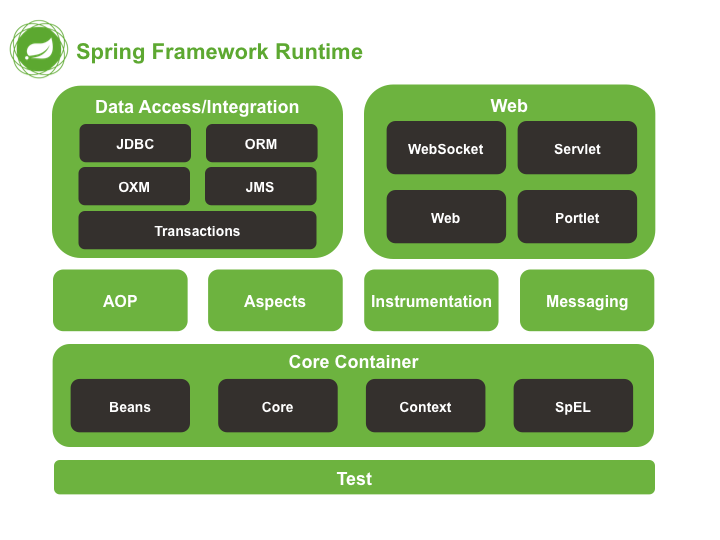
\includegraphics[width=15cm]{img/spring_runtime.png}
  \captionof{figure}{Spring Framework Runtime}
\end{center}

\subsubsubsection{Điểm mạnh của Framework Spring}

Dưới đây là danh sách các lợi ích tuyệt vời của việc sử dụng Spring Framework:
\begin{itemize}
    \item Spring cho phép các nhà phát triển tạo các ứng dụng cấp Enterprise sử dụng các POJO. Lợi ích của việc sử dụng các POJO là bạn không cần một sản phẩm chứa EJB như một máy chủ ứng dụng, mà bạn chỉ có thể sử dụng một bộ chứa servlet mạnh mẽ như Tomcat hoặc một số sản phẩm thương mại khác.
    \item Spring được tổ chức theo kiểu mô đun. Mặc dù số lượng các gói và các lớp là khá nhiều, nhưng bạn chỉ cần quan tâm đến những gì bạn cần và không cần quan tâm đến phần còn lại.
    \item Spring sử dụng một số công nghệ hiện có như một số ORM Framework, logging frameworks, JEE, Quartz, JDK timers và các công nghệ View khác.
    \item Dễ dàng để kiểm thử một chương trình được viết bằng Spring.
    \item Web framework của Spring là một Web MVC framework có thiết kế tốt, nó là một thay thế tuyệt vời cho Struts và các công nghệ kém phổ biến khác.
    \item Spring cung cấp một API thuận tiện để dịch các ngoại lệ công nghệ cụ thể (ném bởi JDBC, Hibernate, hoặc JDO chẳng hạn) vào các trường hợp ngoại lệ nhất quán, không được kiểm soát.
    \item IoC Container có trọng lượng nhẹ. Điều này có lợi cho việc phát triển và triển khai các ứng dụng trên các máy tính có bộ nhớ và tài nguyên CPU hạn chế.
    \item Spring cung cấp một giao diện quản lý transaction nhất quán có thể mở rộng đến một local transaction (ví dụ như sử dụng một cơ sở dữ liệu) và mở rộng lên các global transaction (sử dụng JTA).
\end{itemize}
\subsubsection{Python}
\subsubsubsection{Python là gì}

\begin{center}
  \captionsetup{type=figure}
  \includesvg[width=10cm]{img/python.svg}
  \captionof{figure}{Python}
\end{center}

Python là một ngôn ngữ thông dịch bậc cao, đa mục đích được tạo bởi Guido van Rossum vào năm 1991. Python được thiết kế với ưu điểm mạnh là dễ đọc, dễ học và dễ nhớ. Python là ngôn ngữ có hình thức rất sáng sủa, cấu trúc rõ ràng, thuận tiện cho người mới học lập trình. Cấu trúc của Python còn cho phép người sử dụng viết mã lệnh với số lần gõ phím tối thiểu.
\subsubsubsection{Đặc điểm của Python}
\begin{itemize}
    \item \textbf{Ngôn ngữ lập trình đơn giản, dễ học:} Python có cú pháp rất đơn giản, rõ ràng. Nó dễ đọc và viết hơn rất nhiều khi so sánh với những ngôn ngữ lập trình khác như C++, Java, C\#. Python làm cho việc lập trình trở nên thú vị, cho phép bạn tập trung vào những giải pháp chứ không phải cú pháp.
    \item \textbf{Miễn phí, mã nguồn mở:} Bạn có thể tự do sử dụng và phân phối Python, thậm chí là dùng cho mục đích thương mại. Vì là mã nguồn mở, bạn không những có thể sử dụng các phần mềm, chương trình được viết trong Python mà còn có thể thay đổi mã nguồn của nó. Python có một cộng đồng rộng lớn, không ngừng cải thiện nó mỗi lần cập nhật.
    \item \textbf{Khả năng di chuyển:} Các chương trình Python có thể di chuyển từ nền tảng này sang nền tảng khác và chạy nó mà không có bất kỳ thay đổi nào. Nó chạy liền mạch trên hầu hết tất cả các nền tảng như Windows, MacOS, Linux.
    \item \textbf{Khả năng mở rộng và có thể nhúng:} Giả sử một ứng dụng đòi hỏi sự phức tạp rất lớn, bạn có thể dễ dàng kết hợp các phần code bằng C, C++ và những ngôn ngữ khác (có thể gọi được từ C) vào code Python. Điều này sẽ cung cấp cho ứng dụng của bạn những tính năng tốt hơn cũng như khả năng scripting mà những ngôn ngữ lập trình khác khó có thể làm được.
    \item \textbf{Ngôn ngữ thông dịch cấp cao:} Không giống như C/C++, với Python, bạn không phải lo lắng những nhiệm vụ khó khăn như quản lý bộ nhớ, dọn dẹp những dữ liệu vô nghĩa,... Khi chạy code Python, nó sẽ tự động chuyển đổi code sang ngôn ngữ máy tính có thể hiểu. Bạn không cần lo lắng về bất kỳ hoạt động ở cấp thấp nào.
    \item \textbf{Thư viện tiêu chuẩn lớn để giải quyết những tác vụ phổ biến:} Python có một số lượng lớn thư viện tiêu chuẩn giúp cho công việc lập trình của bạn trở nên dễ thở hơn rất nhiều, đơn giản vì không phải tự viết tất cả code. Ví dụ: Bạn cần kết nối cơ sở dữ liệu MySQL trên Web server? Bạn có thể nhập thư viện MySQLdb và sử dụng nó. Những thư viện này được kiểm tra kỹ lưỡng và được sử dụng bởi hàng trăm người. Vì vậy, bạn có thể chắc chắn rằng nó sẽ không làm hỏng code hay ứng dụng của mình.
    \item \textbf{Hướng đối tượng:} Mọi thứ trong Python đều là hướng đối tượng. Lập trình hướng đối tượng (OOP) giúp giải quyết những vấn đề phức tạp một cách trực quan. Với OOP, bạn có thể phân chia những vấn đề phức tạp thành những tập nhỏ hơn bằng cách tạo ra các đối tượng.
\end{itemize}
\subsubsubsection{Python được dùng ở đâu?}
\begin{itemize}
    \item \textbf{Lập trình ứng dụng web:} Ta có thể tạo web app có khả năng mở rộng (scalable) được bằng cách sử dụng framework và CMS (Hệ thống quản trị nội dung) được tích hợp trong Python. Vài nền tảng phổ biến để tạo web app là:  Django, Flask, Pyramid, Plone, Django CMS. Các trang như Mozilla, Reddit, Instagram và PBS đều được viết bằng Python.
    \item \textbf{Khoa học và tính toán:} Có nhiều thư viện trong Python cho khoa học và tính toán số liệu, như SciPy và NumPy, được sử dụng cho những mục đích chung chung trong tính toán. Và, có những thư viện cụ thể như: EarthPy cho khoa học trái đất, AstroPy cho Thiên văn học,... Ngoài ra, Python còn được sử dụng nhiều trong machine learning, khai thác dữ liệu và deep learning.
    \item \textbf{Tạo nguyên mẫu phần mềm:} Python chậm hơn khi so sánh với các ngôn ngữ được biên dịch như C++ và Java. Nó có thể không phải là lựa chọn tốt nếu nguồn lực bị giới hạn và yêu cầu về hiệu quả là bắt buộc. Tuy nhiên, Python là ngôn ngữ tuyệt vời để tạo những nguyên mẫu (bản chạy thử - prototype). Ví dụ, bạn có thể sử dụng Pygame (thư viện viết game) để tạo nguyên mẫu game trước. Nếu thích nguyên mẫu đó có thể dùng C++ để viết game thực sự.
    \item \textbf{Ngôn ngữ tốt để dạy lập trình:} Python được nhiều công ty, trường học sử dụng để dạy lập trình cho trẻ em và những người mới lần đầu học lập trình. Bên cạnh những tính năng và khả năng tuyệt vời thì cú pháp đơn giản và dễ sử dụng của nó là lý do chính cho việc này.
\end{itemize}
\subsubsubsection{Thế mạnh của Python}
\begin{itemize}
  \item \textbf{Đơn giản:} Cú pháp đơn giản giúp cho người lập trình dễ dàng đọc và tìm hiểu.
  \item \textbf{Tốc độ:} Python có tốc độ xử lý nhanh hơn so với ngôn ngữ PHP.
  \item \textbf{Tương tác:} Chế độ tương tác cho phép người lập trình thử nghiệm tương tác sửa lỗi của các đoạn mã.
  \item \textbf{Chất lượng:} Thư viện có tiêu chuẩn cao, Python có khối cơ sở dữ liệu khá lớn nhằm cung cấp giao diện cho tất cả các CSDL thương mại lớn.
  \item \textbf{Thuận tiện:} Python được biên dịch và chạy trên tất cả các nền tảng lớn hiện nay.
  \item \textbf{Mở rộng:} Với tính năng này, Python cho phép người lập trình có thể thêm hoặc tùy chỉnh các công cụ nhằm tối đa hiệu quả có thể đạt được trong công việc.
\end{itemize}
\subsubsubsection{Framework Django}
\begin{center}
  \captionsetup{type=figure}
  
\includegraphics[width=15cm]{img/django.png}
  \captionof{figure}{Django}
\end{center}

Django là một web framework miễn phí mã nguồn mở được viết bằng Python. Django sử dụng mô hình Model-View-Control (MVC). Django được phát triển bởi Django Software Foundation(DSF) – một tổ chức phi lợi nhuận độc lập.

Mục tiêu chính của Django là đơn giản hóa việc tạo các website phức tạp có sử dụng cơ sở dữ liệu. Django tập trung vào tính năng “có thể tái sử dụng” và “có thể tự chạy” của các component, tính năng phát triển nhanh, không làm lại những gì đã làm. Một số website phổ biến được xây dựng từ Django là Pinterest, Instagram, Mozilla, và Bitbucket.

Django là một trong những framework phát triển web được yêu thích nhất cho việc phát triển các ứng dụng Python. Framework Django cho phép nguyên lý DRY (Don't Repeat Yourself) 

Không như các framework khácc, framework full-stack sử dụng miễn phí và mã nguồn mở của Python bao gồm một số lượng lớn các tính năng tích hợp thay vì cung cấp chúng dưới dạng các thư viện riêng lẻ. Django sử dụng ORM của nó để ánh xạ các đối tượng vào các bảng cơ sở dữ liệu. Điều này cho phép code hoạt động trên các cơ sở dữ liệu khác nhau cũng như giúp việc di chuyển từ cơ sở dữ liệu này sang cơ sở dữ liệu khác dễ dàng hơn. Mặc dù Django có hỗ trợ cho MySQL, PostgreSQL, SQLite và Oracle Database, nhưng nó vẫn có thể hỗ trợ các cơ sở dữ liệu khác thông qua trình điều khiển của bên thứ ba.

\textbf{Các điểm nổi bật chính:}
\begin{itemize}
    \item Học tập nhanh. Tương tự Python, Django cũng rất dễ học, không như Ruby on Rails.
    \item Tự động tạo SQL tables. Django sẽ thay bạn làm công việc này khi bạn đã xác định được cấu trúc.
    \item Tạo forms. Khi bạn đã tạo được Form class trong Django và linked đến model, form generator trong Django sẽ đảm nhận render form, xác minh và lưu trưc data.
    \item Admin Interface. Tương tự SQL table, khi bạn đã xác định được cấu trúc, Django sẽ tạo một admin interface cho phép bạn quản lý database (không khác gì PhpMyAdmin được build-in trong Django cả.)
    \item Django Shell. Python shell, ngay trong môi trường của Django project, chính là lợi thế mà Django shell mang lại. Tính năng này rất hữu hiệu khi debug (thường khó thực hiện trên PHP hơn).
\end{itemize}

\subsubsubsection{Framework Flask}
\begin{center}
  \captionsetup{type=figure}
  
\includegraphics[width=15cm]{img/flask.png}
  \captionof{figure}{Flask}
\end{center}

Flask là một web frameworks, nó thuộc loại micro-framework được xây dựng bằng ngôn ngữ lập trình Python. Flask cho phép bạn xây dựng các ứng dụng web từ đơn giản tới phức tạp. Nó có thể xây dựng các api nhỏ, ứng dụng web chẳng hạn như các trang web, blog, trang wiki hoặc một website dựa theo thời gian hay thậm chí là một trang web thương mại. Flask cung cấp cho bạn công cụ, các thư viện và các công nghệ hỗ trợ bạn làm những công việc trên.

Flask là một micro-framework. Điều này có nghĩa Flask là một môi trường độc lập, ít sử dụng các thư viện khác bên ngoài. Do vậy, Flask có ưu điểm là nhẹ, có rất ít lỗi do ít bị phụ thuộc cũng như dễ dàng phát hiện và xử lý các lỗi bảo mật.

\textbf{Tính năng của Framework Flask:}
\begin{itemize}
    \item Phát triển máy chủ.
    \item Phát triển trình gỡ lỗi.
    \item Hỗ trợ sẵn sàng để kiểm thử đơn vị.
    \item Jinja2 templates.
    \item RESTful request dispatch.
    \item Hỗ trợ bảo mật cookie.
    \item Full WSGI compliant.
    \item Tài liệu mở rộng.
    \item Dựa trên Unicode.
    \item Khả năng tương thích công cụ dựa trên ứng dụng Google.
    \item Nhiều tiện ích mở rộng cho các tính năng mong muốn.
    \item Tính modular và thiết kế gọn nhẹ.
    \item ORM-agnostic.
    \item Độ linh hoạt cao.
    \item Cung cấp xử lý HTTP request.
    \item API có độc đáo và mạch lạc.
    \item Dễ dàng triển khai.
\end{itemize}

\textbf{Điểm mạnh của Framework Flask:}
\begin{itemize}
  \item \textbf{Flask là một micro web framework:} Flask là một micro web framework được viết bằng Python, không yêu cầu tool hay thư viện cụ thể nào. “Micro” không có nghĩa là thiếu chức năng mà “micro” theo triết lý thiết kế là cung cấp một lõi chức năng “súc tích” nhất cho ứng dụng web nhưng người dùng có thể mở rộng bất cứ lúc nào. Flask luôn hỗ trợ các thành phần tiện ích mở rộng cho ứng dụng như tích hợp cơ sở dữ liệu, xác thực biểu mẫu, xử lý upload, các công nghệ xác thực, template, email, RESTful..., chỉ khác là khi nào bạn muốn thì bạn mới đưa vào thôi. Người dùng có thể tập trung xây dựng web application ngay từ đầu trong một khoảng thời gian rất ngắn và có thể phát triển quy mô của ứng dụng tùy theo yêu cầu.
  \item \textbf{Flask dễ cài đặt và triển khai:} Sau khi cài đặt Python, để cài đặt Flask chỉ cần bạn gõ lệnh: pip install Flask Bây giờ chúng ta thử tạo ứng dụng web với câu chào Hello World!. Thật đơn giản bạn sẽ tạo một folder với tên folder là tên ứng dụng, sau đó, tạo một tập tin .py và viết code. Flask tập trung vào sự tối giản, cho phép chúng ta xây dựng ứng dụng nhanh hơn.
  \item \textbf{Flask thật sự phù hợp cho việc xây dựng các web application có quy mô vừa và nhỏ, các API và web services:} 
  \begin{itemize}
    \item Xây dựng web application rất giống với việc viết các module Python chuẩn, cấu trúc gọn gàng và rõ ràng.
    \item Thay vì cung cấp hết tất cả mọi thứ, Flask cung cấp cho người dùng các thành phần cốt lõi thường được sử dụng nhất của khung ứng dụng web như URL routing, request and response object, template...
    \item Với Flask, việc chọn component nào cho ứng dụng là việc của chúng ta. Điều này thật tuyệt, vì mỗi web application có những đặc điểm và tính năng riêng, nó không phần phải chứa các component mà nó không dùng.
\end{itemize}
  \item \textbf{Flask giúp ta tập trung xây dựng ý tưởng, mục tiêu của riêng mình:} Flask có kiến trúc nhỏ, gọn nên bạn hoàn toàn không bị bó buộc bởi bộ khung cồng kềnh, không gặp bất cứ khó khăn nào khi cấu hình hay tổ chức ứng dụng. Không những thế, Flask còn có các ưu điểm nổi bật như: cực kỳ linh hoạt, tối giản, dễ tìm hiểu và sử dụng, định tuyến dễ dàng, rất dễ mở rộng. Vì vậy, công việc chính của ta là chỉ cần xác định ý tưởng, mục tiêu, tập trung vào việc xây dựng ứng dụng web mà thôi.
  \item \textbf{Nguồn tài liệu tham khảo về Flask rất phong phú:} Flask cung cấp rất nhiều tài liệu từ cài đặt đến thực hiện và triển khai, từ hướng dẫn nhanh đến hướng dẫn chi tiết. Ta có thể dễ dàng tìm kiếm, tham khảo, học tập về lập trình web application với Flask framework miễn phí trên Internet.
  \item \textbf{Cộng đồng Flask khá lớn:} Ta có thể dễ dàng, nhanh chóng tìm được giải pháp từ cộng đồng người sử dụng Flask mỗi khi gặp vấn đề cần giúp đỡ ví dụ như gặp lỗi, cách cài đặt thư viện, cách triển khai ứng dụng.
  \item \textbf{Mức độ phổ biến:} Có nhiều khách hàng đặt web application được xây dựng từ Flask Framework như Pinterest, LinkedIn, Twilio, Reddit, Netflix, Uber…
\end{itemize}
\subsubsection{NodeJS}
\subsubsubsection{NodeJS là gì}

\begin{center}
  \captionsetup{type=figure}
  \includesvg[width=10cm]{img/nodejs.svg}
  \captionof{figure}{NodeJS}
\end{center}


NodeJS là một mã nguồn được xây dựng dựa trên nền tảng Javascript V8 Engine, nó được sử dụng để xây dựng các ứng dụng web như các trang video clip, các forum và đặc biệt là trang mạng xã hội phạm vi hẹp. NodeJS là một mã nguồn mở được sử dụng rộng bởi hàng ngàn lập trình viên trên toàn thế giới. NodeJS có thể chạy trên nhiều nền tảng hệ điều hành khác nhau từ Windows cho tới Linux, OSX nên đó cũng là một lợi thế. NodeJS cung cấp các thư viện phong phú ở dạng Javascript module khác nhau giúp đơn giản hóa việc lập trình và giảm thời gian ở mức thấp nhất.

\subsubsubsection{Đặc điểm của NodeJS}

\begin{itemize}
  \item \textbf{Realtime:} Đây là tính năng quan trọng nhất của NodeJS. Realtime ở đây chính là xử lý giao tiếp từ client tới máy chủ theo thời gian thực. Giống như khi bạn lướt Facebook thì mỗi khi bạn comment hay like một topic nào đó thì ngay lập tức chủ topic và những người đã comment trên đó sẽ nhận được thông báo là bạn đã comment.
  \item \textbf{Không đồng bộ:} Tất cả các API của NodeJS đều không đồng bộ (none-blocking), nó chủ yếu dựa trên nền của NodeJS Server và chờ đợi Server trả dữ liệu về. Việc di chuyển máy chủ đến các API tiếp theo sau khi gọi và cơ chế thông báo các sự kiện của Node.js giúp máy chủ để có được một phản ứng từ các cuộc gọi API trước (Realtime).
  \item \textbf{Chạy rất nhanh:} NodeJ được xây dựng dựa vào nền tảng V8 Javascript Engine nên việc thực thi chương trình rất nhanh.
  \item \textbf{Đơn luồng nhưng khả năng mở rộng cao:} Node.js sử dụng một mô hình luồng duy nhất với sự kiện lặp. cơ chế tổ chức sự kiện giúp các máy chủ để đáp ứng một cách không ngăn chặn và làm cho máy chủ cao khả năng mở rộng như trái ngược với các máy chủ truyền thống mà tạo đề hạn chế để xử lý yêu cầu. Node.js sử dụng một chương trình đơn luồng và các chương trình tương tự có thể cung cấp dịch vụ cho một số lượng lớn hơn nhiều so với yêu cầu máy chủ truyền thống như Apache HTTP Server.
  \item \textbf{Không đệm:} NodeJS không đệm bất kì một dữ liệu nào và các ứng dụng này chủ yếu là đầu ra dữ liệu.
  \item \textbf{Có giấy phép:} NodeJS đã được cấp giấy phép bởi MIT License.
\end{itemize}

\subsubsubsection{NodeJs được sử dụng ở đâu}
\begin{itemize}
  \item \textbf{Websocket server:} Các máy chủ web socket như là Online Chat, Game Server…
  \item \textbf{Fast File Upload Client:} Là các chương trình upload file tốc độ cao.
  \item \textbf{Ad Server:} Các máy chủ quảng cáo.
  \item \textbf{Cloud Services:} Các dịch vụ đám mây.
  \item \textbf{RESTful API:} Đây là những ứng dụng mà được sử dụng cho các ứng dụng khác thông qua API.
  \item \textbf{Any Real-time Data Application:} Bất kỳ một ứng dụng nào có yêu cầu về tốc độ thời gian thực. Micro Services: Ý tưởng của micro services là chia nhỏ một ứng dụng lớn thành các dịch vụ nhỏ và kết nối chúng lại với nhau. Nodejs có thể làm tốt điều này.
\end{itemize}

\subsubsubsection{Thế mạnh của NodeJS}
\begin{itemize}
  \item Cú pháp ngắn gọn, dễ nhớ. Đặc biệt dễ học với những ai đã từng làm việc với nhiều với Javascript, Jquery.
  \item Xử lý không đồng bộ tốt: ví dụ khi upload file, chương trình không chờ việc upload xong mới xử lý việc tiếp theo. Nghĩa là trong khi xử lý upload file chương trình vẫn tiếp tục xử lý các công việc mới.
  \item Khả năng xử lý song song tuyệt vời: NodeJs sẽ tận dụng tối đa Unix để hoạt động. Tức là NodeJs có thể xử lý hàng nghìn process và trả ra 1 luồng khiến cho hiệu xuất hoạt động đạt mức tối đa nhất.
  \item Có nhiều packages hỗ trợ để tạo nhiều chức năng cho site, các packages được cài đặt bằng câu lệnh giống như cài đặt gem trong ruby on rails.
  \item Hỗ trợ nhiều template engine để render view.
  \item Có nhiều framework. Được sử dụng phổ biến nhất là : ExpressJs, SailsJS.
  \item Khả năng sử dụng lại code: dễ dàng tạo ra các module, helper, library để sử dụng ở nhiều nơi.
  \item Hỗ trợ security tốt. NodeJs mặc định hỗ trợ chống tấn công Cross-site script.
\end{itemize}

\subsubsubsection{ExpressJS}
\begin{center}
  \captionsetup{type=figure}
  
\includegraphics[width=15cm]{img/expressjs.png}
  \captionof{figure}{Express JS}
\end{center}

Express.js được xây dựng bởi TJ Holowaychuk, một thành viên trong team Node đã tạo ra Node.js. Cũng chính vì vậy mà đây là một trong những framework quan trọng nhất của Node.js. Expressjs cung cấp các hàm HTTP và midleware để tạo ra API đơn giản và dễ sử dụng. Express.js là một framework tối giản để xây dựng một loạt các ứng dụng web và di động cũng như các giao diện lập trình ứng dụng (API). Được ủng hộ bởi một cộng đồng lớn, framework này luôn được cập nhật liên tục và cải thiện tất cả những tính năng cốt lõi. Express.js cung cấp nhiều tính năng khác nhau như đơn giản hóa nhiều định tuyến, tích hợp cơ sở dữ liệu … và nhờ đó được dùng cho những ứng dụng phổ biến trên các trang web như MySpace, Geekli.st, Klout, Segment.io và Yummly.

ExpressJS được phát hành theo giấy phép mã nguồn mở, có cộng đồng hỗ trợ lớn, được phép sử dụng cho ứng dụng có mục đích thương mại.

Cấu trúc thư mục dự án khi sử dụng ExpressJS được chia là 3 phần: routes, Views và Public. ExpressJS xây dựng ứng dụng web theo đúng mô hình MVC (Model - View - Controller).

\textbf{Một số chức năng chính của ExpressJS:}
\begin{itemize}
  \item Hỗ trợ middleware để trả về các HTTP request.
  \item Định nghĩa route dựa trên các action của HTTP (CRUD).
  \item Cho phép trả về các trang html sử dụng các template engine (jade, pug…).
\end{itemize}

\subsubsubsection{Middleware trong ExpressJS:}

Middleware trong ngành công nghệ phần mềm được định nghĩa là một phần mềm có nhiệm vụ làm cầu nối (bridge), cung cấp các dịch vụ từ phía hệ điều hành đến các ứng dụng, giúp các ứng dụng có thể tương tác với các thành phần được hệ điều hành cho phép. Middleware được coi là chất kết dính dữa các phần mềm với nhau.

\textbf{Middleware trong Web:} 

Với tư tưởng chung là cầu nối giữa tương tác của người dùng và phần nhân của hệ thống, trong lập trình Web, Middleware sẽ đóng vai trò trung gian giữa request/response (tương tác với người dùng) và các xử lý logic bên trong web server.Do đó, Middleware trong các Framework lập tình Web (Django, Rails, ExpressJS), sẽ là các hàm được dùng để tiền xử lý, lọc các request trước khi đưa vào xử lý logic hoặc điều chỉnh các response trước khi gửi về cho người dùng.

\begin{center}
  \captionsetup{type=figure}
  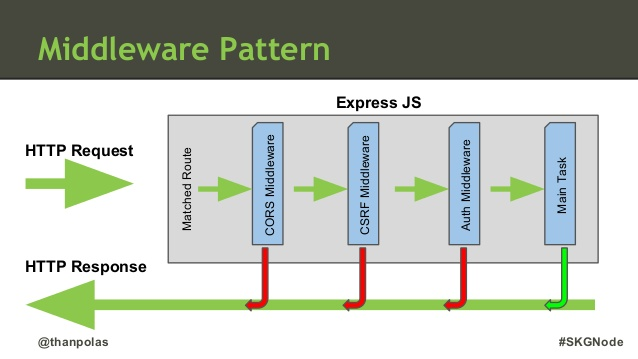
\includegraphics[width=15cm]{img/expressjsmiddleware.jpg}
  \captionof{figure}{Express JS}
\end{center}

Hình trên mô tả 3 middleware có trong ExpressJS. Một request khi gửi đến Express sẽ được xử lý qua 5 bước như sau :
\begin{itemize}
  \item Tìm Route tương ứng với request.
  \item Dùng CORS Middleware để kiểm tra cross-origin Resource sharing của request.
  \item Dùng CRSF Middleware để xác thực CSRF của request, chống fake request.
  \item Dùng Auth Middleware để xác thực request có được truy cập hay không.
  \item Xử lý công việc được yêu cầu bởi request (Main Task).
\end{itemize}

Bất kỳ bước nào trong các bước 2, 3, 4 nếu xảy ra lỗi sẽ trả về response thông báo cho người dùng, có thể là lỗi CORS, lỗi CSRF hay lỗi auth tùy thuộc vào request bị dừng ở bước nào.
\textbf{Middleware trong ExpressJS:} 

ExpressJS khi hoạt động, về cơ bản sẽ là một loạt các hàm Middleware được thực hiện liên tiếp nhau. Sau khi đã thiết lập, các request từ phía người dùng khi gửi lên ExpressJS sẽ thực hiện lần lượt qua các hàm Middleware cho đến khi trả về response cho người dùng. Các hàm này sẽ được quyền truy cập đến các đối tượng đại diện cho Request - req, Response - res, hàm Middleware tiếp theo - next, và đối tượng lỗi - err nếu cần thiết.

Một hàm Middleware sau khi hoạt động xong, nếu chưa phải là cuối cùng trong chuỗi các hàm cần thực hiện, sẽ cần gọi lệnh next() để chuyển sang hàm tiếp theo, bằng không xử lý sẽ bị treo tại hàm đó.

Các chức năng mà middleware có thể thực hiện trong ExpressJS sẽ bao gồm :
\begin{itemize}
  \item Thực hiện bất cứ đoạn code nào.
  \item Thay đổi các đối tượng request và response.
  \item Kết thúc một quá trình request-response.
  \item Gọi hàm middleware tiếp theo trong stack.
\end{itemize}

Trong Express, có 5 kiểu middleware có thể sử dụng :
\begin{itemize}
  \item Application-level middleware (middleware cấp ứng dụng).
  \item Router-level middleware (middlware cấp điều hướng - router).
  \item Error-handling middleware (middleware xử lý lỗi).
  \item Built-in middleware (middleware sẵn có).
  \item Third-party middleware (middleware của bên thứ ba).
\end{itemize}
\subsubsection{Sự lựa chọn}
Pikachu, I choose you

https://www.quora.com/How-is-Node-js-better-than-Java-or-Python-at-the-backend
\subsection{Cơ sở dữ liệu (Database)}
\subsubsection{Hệ cơ sở dữ liệu quan hệ (RDBMS)}
\textbf{Khái niệm:}\\

RDBMS - Relational Database Management System - là hệ cơ sở dữ liệu quan hệ. Tất cả các hệ thống quản trị cơ sở dữ liệu hiện đại như SQL, MySQL, MS SQL Server, Oracle, ... đều dựa trên RDBMS.

Hệ thống quản lý cơ sở dữ liệu quan hệ (RDBMS) là một hệ thống quản lý cơ sở dữ liệu (DBMS) dựa trên mô hình quan hệ được giới thiệu bởi EF Codd.

\textbf{Bảng (Table):}\\

RDBMS sử dụng các bảng để lưu trữ dữ liệu. Mỗi bảng là một tập hợp các dữ liệu có liên quan đến nhau và có nhiều hàng và cột để lưu dữ liệu. Bảng là hình thức lưu trữ phổ biến và đơn giản nhất trong môt cơ sở dữ liệu quan hệ. Ví dụ về bảng một nhóm môn học trong bảng MONHOC sau đây:\\
\begin{table}[!h]
    \centering
    \begin{tabular}{|l|l|l|}
    \hline
         \textbf{ID}&\textbf{TEN\_MON\_HOC}&\textbf{SO\_TIN\_CHI}\\
         \hline
         1&Giải tích 1&4\\
		\hline
		2&Vật lý&3\\
		\hline			
		3&Kỹ thuật lập trình&4\\
		\hline
    \end{tabular}
    \caption{Ví dụ về bảng dữ liệu}
\end{table}

\textbf{Trường (Field):}\\
	
	Mỗi bảng được chia thành các thực thể nhỏ gọi là các trường, chứa các thông tin cụ thể về mỗi bản ghi trong bảng. Các trường trong bảng MONHOC bao gồm: ID, TEN\_MON\_HOC, SO\_TIN\_CHI.\\
	\begin{table}[!h]
	    \centering
	    \begin{tabular}{|l|}
	        \hline
	        \textbf{TEN\_MON\_HOC}\\
	        \hline
	        Giải tích 1\\
	        \hline
	        Vật lý\\
	        \hline
	        Kỹ thuật lập trình\\
	        \hline
	    \end{tabular}
	    \caption{Ví dụ một trường trong bảng dữ liệu}
	\end{table}
	
\textbf{Hàng hoặc bản ghi (Record):}\\
	
Một hàng của bảng được gọi là bản ghi , nó chứa thông tin của một đối tượng trong bảng. Ví dụ ở bảng MONHOC có 3 bản ghi. Sau đây là một bản ghi trong bảng:\\
\begin{table}[!h]
    \centering
    \begin{tabular}{|r|r|r|}
        \hline
		1&Giải tích 1&4\\
		\hline
    \end{tabular}
    \caption{Ví dụ về một bản ghi}
\end{table}

\textbf{Ràng buộc (Constraint):}\\

Ràng buộc là các quy tắc cho các cột dữ liệu trong bảng. Chúng được sử dụng để giới hạn loại dữ liệu có thể insert vào một bảng. Điều này đảm bảo tính chính xác và độ tin cậy của dữ liệu trong cơ sở dữ liệu.\\
Constraint có thể là cấp độ cột hoặc cấp độ bảng. Các ràng buộc cấp độ cột chỉ được áp dụng cho một
cột trong khi các ràng buộc mức bảng được áp dụng cho toàn bộ bảng.\\
Sau đây là một số ràng buộc phổ biến nhất được sử dụng trong SQL :\\
\begin{table}[!h]
    \centering
    \begin{tabular}{|l|l|}
        \hline
         NOT NULL&Đảm bảo rằng một field không có giá trị NULL  \\
         \hline
         DEFAULT&Cung cấp giá trị mặc định của một field khi không được xác định\\
         \hline
         UNIQUE&Đảm bảo giá trị trong một field là khác nhau\\
         \hline
         PRIMARY Key&Mỗi record là duy nhất trong một bảng cơ sở dữ liệu\\
         \hline
         FOREIGN Key&Mỗi record là duy nhất trong trong bất kỳ bảng cơ sở dữ liệu khác\\
         \hline
         CHECK&Đảm bảo rằng tất cả các giá trị trong một cột thỏa mãm một số điều kiện\\
         \hline
         INDEX&Dùng để tạo và lấy dữ liệu một cách nhanh chóng\\
         \hline
    \end{tabular}
    \caption{Một số ràng buộc phổ biến trong SQL}
\end{table}
\subsubsection{Hệ quản trị cơ sở dữ liệu}

Hệ quản trị cơ sở dữ liệu (Database Management System - DBMS) là hệ thống kiểm soát việc lưu trữ, tổ chức và truy xuất dữ liệu.

Mỗi DBMS đều có thành phần gọi là Query Language (Ngôn ngữ truy vấn), các ứng dụng muốn truy cập dữ liệu đều phải nhờ vào thành phần này.

Các hệ quản trị cơ sở dữ liệu quan hệ phổ biến nhất hiện nay:
\subsubsubsection{Oracle Database}
\begin{figure}[!h]
    \centering
    
\includegraphics[scale=0.4]{img/oracle.jpg}
    \caption{Oracle Database}
\end{figure}

Oracle Database hay còn gọi là Oracle RDBMS hoặc đơn giản là Oracle là 1 hệ quản trị cơ sở dữ liệu quan hệ, được phát triển và phân phối bởi tập đoàn Oracle.\\

\textit{Đặc điểm và thế mạnh:}
\begin{itemize}
    \item Quản lý được hệ thống dữ liệu lớn
    \item Hỗ trợ nhiều công cụ để quản trị cũng như nhập, xuất dữ liệu dễ dàng
    \item Có thể hoạt động trên nhiều hệ điều hành khác nhau như Windows, Linux, Mac OS, Unix,...
    \item Truy cập đồng thời
    \item Hỗ trợ cơ chế khóa
    \item Thực thi song song
    \item Tính khả chuyển
\end{itemize}

\subsubsubsection{MySQL}
\begin{figure}[!h]
    \centering
    
\includegraphics[scale=0.5]{img/mysql.jpg}
    \caption{MySQL}
\end{figure}

MySQL là một hệ quản trị cơ sở dữ liệu quan hệ mã nguồn mở, được phát triển, phân phối và hỗ trợ bởi tập đoàn Oracle.\\

\textit{Đặc điểm và thế mạnh:}
\begin{itemize}
    \item \textbf{Tính nội bộ và linh động:}
    \begin{itemize}
    \item Viết bằng C và C++
    \item Đã thử nghiệm với một loạt các trình biên dịch khác nhau
    \item Hoạt động trên nhiều nền tảng khác nhau
    \item Sử dụng thiết kế máy chủ nhiều lớp với các mo-đun độc lập
    \item Được thiết kế để đa luồng hoàn toàn bằng cách sử dụng các luồng nhân, để dễ dàng sử dụng nhiều CPU nếu chúng có sẵn
    \item Triển khai các bảng băm trong bộ nhớ, được sử dụng làm bảng tạm thời.
    \item Triển khai các hàm SQL bằng cách sử dụng thư viện lớp được tối ưu hóa cao nhất phải nhanh nhất có thể
    \end{itemize}
    \item \textbf{Bảo mật}
    \begin{itemize}
        \item Một hệ thống đặc quyền và mật khẩu rất linh hoạt và an toàn, và cho phép xác minh dựa trên máy chủ
        \item Bảo mật mật khẩu bằng cách mã hóa tất cả lưu lượng mật khẩu khi bạn kết nối với máy chủ.
    \end{itemize}
    \item \textbf{Khả năng mở rộng và giới hạn:}
    \begin{itemize}
        \item Hỗ trợ cơ sở dữ liệu lớn
        \item Hỗ trợ lên đến 64 chỉ mục cho mỗi bảng
    \end{itemize}
    \item \textbf{Ổn định, có tốc độ cao và dễ sử dụng}
    \item \textbf{Đa tính năng:} Hỗ trợ rất nhiều chức năng SQL
\end{itemize}
\subsubsubsection{SQL Server}
\begin{figure}[!h]
    \centering
    
\includegraphics[scale=0.3]{img/sql-server.png}
    \caption{SQL Server}
\end{figure}
SQL Server là một RDBMS được phát triển bởi tập đoàn Microsoft.\\

\textit{Thế mạnh:}
\begin{itemize}
    \item Cho phép nhiều người dùng chung một cơ sở dữ liệu
    \item Duy trì lưu trữ bền vững
    \item Khả năng mở rộng
    \item Tính bảo mật cao
    \item Độ tin cậy, bảo vệ dữ liệu
    \item Hỗ trợ phân tích dữ liệu
    \item Kết hợp tốt với các sản phẩm của Microsoft
\end{itemize}

\subsubsubsection{PostgreSQL}
\begin{figure}[!h]
    \centering
    
\includegraphics[scale=0.5]{img/postgre-sql.jpg}
    \caption{PostgreSQL}
\end{figure}

PostgreSQL là một RDBMS mở nguồn mở được xây dựng trên mã nguồn ban đầu của đại học Berkeley.\\

\textit{Đặc điểm và thế mạnh:}
\begin{itemize}
    \item Truy xuất dữ liệu tốc độ nhanh
    \item Sử dụng câu truy vấn phức tạp
    \item Sử dụng khóa ngoại
    \item Có thủ tục
    \item Đảm bảo tính toàn vẹn của các giao tác
\end{itemize}

\subsubsection{Hệ cơ sở dữ liệu phi quan hệ (Non-RDBMS)}
Hệ cơ sở dữ liệu phi quan hệ là cơ sở dữ liệu không sử dụng mô hình bảng gồm các cột và hàng như nhiều hệ cơ sở dữ liệu truyền thống. Thay vào đó, Non-RDBMS sử dụng mô hình lưu trữ được tối ưu hóa cho các yêu cầu cụ thể của loại dữ liệu được lưu trữ. Cơ sở dữ liệu phi quan hệ (Non-relational database) phổ biến nhất được gọi là NoSQL.\\
Các Non-RDBMS phổ biến:
\subsubsubsection{MongoDB}
\begin{center}
  \captionsetup{type=figure}
    
\includegraphics[width=10cm]{img/mongo.png}
  \captionof{figure}{MongoDB}
\end{center}

MongoDB là một hệ quản trị cơ sở dữ liệu mã nguồn mở và là cơ sở dữ liệu NoSQL hàng đầu, được nhiều người sử dụng.

Các thuật ngữ thường sử dụng trong MongoDB:
\begin{itemize}
    \item \textbf{\_id:} Là trường bắt buộc có trong mỗi document. Trường \_id đại diện cho một giá trị duy nhất trong document MongoDB. Trường \_id cũng có thể được hiểu là khóa chính trong document. Nếu bạn thêm mới một document thì MongoDB sẽ tự động sinh ra một \_id.
    \item \textbf{Collection:} Là nhóm của nhiều document trong MongoDB, tương ứng với một bảng trong RDBMS
    \item \textbf{Cursor:} Đây là một con trỏ đến tập kết quả của một truy vấn. Máy khách có thể lặp qua một con trỏ để lấy kết quả.
    \item \textbf{Database:} Nơi chứa các Collection.
    \item \textbf{Document:} Là một bản ghi thuộc một Collection.
    \item \textbf{Field:} Là một cặp name-value trong một document.
\end{itemize}

\textit{Thế mạnh:}
\begin{itemize}
    \item Ít schema hơn
    \item Cấu trúc của một đối tượng rõ ràng
    \item Không có các phép join phức tạp
    \item Khả năng mở rộng cực lớn: Việc mở rộng dữ liệu mà không cần phải quan tâm đến các vấn đề như khóa ngoại, khóa chính, kiểm tra ràng buộc,...
    \item Sử dụng bộ nhớ trong để lưu giữ cửa sổ làm việc cho phép truy cập dữ liệu nhanh hơn. Việc cập nhật được thực hiện nhanh gọn nhờ update tại chỗ (in-place).
\end{itemize}
\subsubsubsection{Neo4j}
\begin{center}
  \captionsetup{type=figure}
  
\includegraphics[width=10cm]{img/neo4j.png}
  \captionof{figure}{Neo4j}
\end{center}

Neo4j là hệ quản trị cơ sở dữ liệu đồ thị đầu tiên được giới thiệu vào năm 2007 và công bố phiên bản 1.0 vào năm 2010. Hiện nay Neo4j là một trong những hệ quản trị cơ sở dữ liệu đồ thị được sử dụng nhiều nhất.\\

\textit{Đặc điểm:} Các đối tượng được miêu tả dưới dạng các đỉnh của đồ thị, các thuộc tính của đối tượng được miêu tả bằng liên kết có hướng đến một đối tượng khác.\\

\textit{Thế mạnh:}
\begin{itemize}
    \item Khả năng mở rộng cao
    \item Phân tích dữ liệu theo thời gian thực
    \item Thời gian thực thi nhanh
\end{itemize}
\subsubsubsection{Cassandra}
\begin{center}
  \captionsetup{type=figure}
  
\includegraphics[width=10cm]{img/cassandra.png}
  \captionof{figure}{Cassandra}
\end{center}

Cassandra ban đầu được tạo ra bởi Facebook. Sau đó nó đã được tặng cho Quỹ Apache và tháng 2 năm 2010 và được nâng cấp lên thành dự án hàng đầu của Apache. Cassandra là một cơ sở dữ liệu phân tán kết hợp mô hình dữ liệu của Google Bigtable với thiết kế hệ thống phân tán như bản sao của Amazon Dynamo.\\

\textit{Đặc điểm:}
\begin{itemize}
    \item Tính phân tán và không tập trung (distributed and decentralized): Khả năng phân chia dữ liệu thành nhiều phần, đặt trên nhiều node khác nhau trong khi người dùng vẫn nhận thấy dữ liệu này là một khối thống nhất.
    \item Tính mềm dẻo (elastic scalability): Hệ thống có thể dễ dàng mở rộng số node trong cluster để có thể phục vụ số lượng request lớn và rút bớt số node khi số lượng request giảm.
\end{itemize}
\subsubsection{So sánh Relational Database và Non-Relational Database}
\begin{table}[!h]
	    \centering
	    \begin{tabular}{|p{3cm}|p{6cm}|p{6cm}|}
	        \hline
	        &\textbf{Relational}&\textbf{Non-Relational}\\
	        \hline
	        Ngôn ngữ truy vấn&Ngôn ngữ truy vấn có cấu trúc &Truy vấn đối tượng: trực quan, chuyển một tài liệu để giải thích những gì bạn đang truy vấn\\
	        \hline
	        Kiểu dữ liệu&Lưu các kiểu dữ liệu được quy định&Có thể lưu bất kỳ loại dữ liệu nào\\
	        \hline
	        Khả năng mở rộng&Mở rộng thêm chiều dọc&Mở rộng theo chiều ngang\\
	        \hline
	        Hiển thị dữ liệu&Dưới dạng bảng và hàng&Dưới dạng JSON\\
	        \hline
	        Chi phí&Chi phí xây dựng và bảo trì cao&Khoảng 10\% so với Relational\\
	        \hline
	    \end{tabular}
	    \caption{So sánh cơ sở dữ liệu quan hệ và cơ sở dữ liệu phi quan hệ}
	\end{table}
	
	
Nội dung cần có:\\
SQL là gì, tính năng, thế mạnh, ...\\
|    SQL server (hình ảnh, là gì, đặc điểm, thế mạnh)\\
|    Oracle     (...)\\
|    MySQL      (...)\\
NoSQL là gì, tính năng, thế mạnh\\
|    MongoDB    (...)\\
|    Neo4j      (...)\\
|    Cassandra, tham khảo: \url{https://drive.google.com/open?id=1jM9vy5ExhZ1IROXV1J8gvoJrT_F64OYw}\\
So sánh SQL, NoSQL\\
m có thể làm 1 folder 7 rồi chia từng phần ra từng file cho dễ làmc
\section{Thiết kế hệ thống}
\subsection{Kiến trúc hệ thống}

\newpage
\begin{thebibliography}{80}

\bibitem{}
\url{https://nodejs.org/en/docs/}, ngày truy cập: 18/12/2019

\bibitem{}
\url{https://docs.oracle.com/en/java/}, ngày truy cập: 18/12/2019

\bibitem{}
\url{https://docs.python.org/3/}, ngày truy cập: 18/12/2019

\bibitem{}
\url{https://docs.djangoproject.com/en/3.0/}, ngày truy cập: 18/12/2019

\bibitem{}
\url{https://hoclaptrinh.vn/posts/django-la-gi}, ngày truy cập: 18/12/2019

\bibitem{}
\url{https://techmaster.vn/posts/35345/cac-framework-trong-python-nam-2019}, ngày truy cập: 18/12/2019

\bibitem{}
\url{http://flask.palletsprojects.com/en/1.1.x/}, ngày truy cập 18/12/2019


\bibitem{}
\url{https://sass-lang.com/}, ngày truy cập: 19/12/2019

\bibitem{}
\url{http://lesscss.org/}, ngày truy cập: 19/12/2019

\bibitem{}
\url{https://docs.mongodb.com/}, ngày truy cập: 20/12/2019

\bibitem{}
\url{https://docs.oracle.com/en/database/oracle/oracle-database/19/cncpt/introduction-to-oracle-database.html}, ngày truy cập: 20/12/2019

\bibitem{}
\url{https://spring.io/docs}, ngày truy cập: 20/12/2019

\bibitem{}
\url{https://dev.mysql.com/doc/refman/8.0/en/}, ngày truy cập: 20/12/2019

\bibitem{}
\url{https://restfulapi.net/}, ngày truy cập: 4/7/2020

\end{thebibliography}

%%%%%%%%%%%%%%%%%%%%%%%%%%%%%%%%%



\end{document}